\documentclass[../thesis.tex]{subfiles}

\begin{document}
\chapter{Numerical results for the control problem}
\label{sec:numerical-results}
In \cref{sec:st-numerics} we presented various numerical approaches for the optimal control problems analyzed in \cref{sec:Disc-Control-Problem}.
The methods were implemented by the author and we want to show numerical results in this chapter.
Before exhibiting said results, we want to discuss how they were implemented.
\section{Implementation notes}
The implementation at hand works for two space dimensions and one time dimension, rendering $Q$ an overall three dimensional domain.
Therefore, the discontinuous Galerkin method operates on tetrahedral meshes.

In order to generate these meshes, a uniform refinement approach was made. The starting mesh was generated by working with prisms to cover $Q$. This way, if the space domain $\Omega$ can be decomposed into triangles, one can cover the space-time domain $Q$ using prisms based on those triangles.
One can quickly verify that a prism can be decomposed into three tetrahedrons. Overall, this approach permits a flexible mesh generation for this problem if one can represent $\Omega$ using triangles.
However, special attention has to be paid when gluing these prisms together to a tetrahedral mesh, as each face of a prism will consist out of two triangles and these must match the next prism in order to obtain a conformal mesh.

Starting from the mesh generated like this, a uniform refinement approach was made to obtain a finer mesh. It would of course be possible to use an adaptive refinement as well, the discontinuous Galerkin method from \cref{sec:dG-method} permits such.
However, it's not clear how an adaptive refinement would be best approached, as one needs to use the same ansatz space $\Shp(\meshT_N)$ for both the state and the adjoint state, at least if one wants to operate in a fashion that is backed by theory. Therefore, any adaptive refinement would have to account for the errors encountered in both the state and the adjoint state at the same time.

In order to ensure that the refined mesh does not become degenerate - keep the strong dependence of mesh specific constants in the error estimates from \cref{sec:dG-numerics} in mind - one has to use a refinement algorithm that ensures such.
The choice employed for this implementation stems from \cite{Bey}. As we only want to use uniform refinements, the algorithm \verb+RegularRefinement+ defined in \cite[p.\ 361]{Bey} is the choice that was made.
For this algorithm, one can show that the refined tetrahedrons belong to at most three congruence classes, see \cite[Theorem  1, p.\ 361]{Bey} for this statement and its proof.
Combined with the generation of the initial mesh, one can see that this approach will result in a total amount of congruence classes of at most nine times the congruence classes of the initial triangulation:
The prism associated with each triangle is decomposed into three tetrahedrons that in turn will yield at most three congruence classes each.
The work \cite{Bey} also incorporates an algorithm that can handle adaptive refinement, which with one could extend this implementation.

As a next step, we have to define a suitable basis $\{ \varphi_j \}_{j=1}^m$ for $\Shp(\meshT_N)$. By employing the common approach of using a reference tetrahedron and an affine linear map, we can obtain such a basis that is a nodal one over that.
One can easily calculate such a map, see also \cite[p.\ 254]{JungLanger}.
Our goal is to be able to use both linear and quadratic bases.
Establishing a nodal basis on the reference tetrahedron can be manually done by picking a number of points on the reference tetrahedron and calculating functions that fit the requirements. The results of such a calculation can be found in \cite[Tabelle 4.4, p.\ 257]{JungLanger}.

Moreover, one needs numerical integration formulas, so that the integrals that appear in $A(\cdot, \cdot)$ can be evaluated. This holds especially true given that the right hand side of \cref{eq:dg-discrete-prob} depends on the specific input of boundary and initial conditions, which do not have to be functions of $\Shp(\meshT_N)$ of course.
A variety of suitable integration formulas for tetrahedral elements is given in \cite[Tabelle 4.15, p.\ 314]{JungLanger}. For the interface terms appearing in $A(\cdot, \cdot)$ we will also need integration formulas for triangles, see \cite[Tabelle 4.14, p.\ 313]{JungLanger} for possible choices.
Either way, we need to integrate the terms of $A(\cdot, \cdot)$ in an exact fashion if we want to apply the theoretical results from \cref{sec:Disc-Control-Problem}. This means that if we denote by $p$ the polynomial degree which $\Shp(\meshT_N)$ uses per element, we need to integrate on the tetrahedrons functions of degree $2p - 2$ for $a^\sip$ and $2p - 1$ for $b$. On the interfaces we need exact precision for polynomial degree $2p$ for all of $a^\sip$, $a^R$ and $b$.
Hence, we can select the following formulas from \cite{JungLanger}:
\begin{itemize}
\item For linear basis functions: ``3DT-1'' on the tetrahedrons, exact for polynomial degree $1 = 2 \cdot 1 - 1$. ``2DD-3'' or ``2DD-4'' on the triangular interfaces, exact for polynomial degree $2 = 2 \cdot 1$.
\item For quadratic basis functions: ``3DT-4'' on the tetrahedrons, exact for polynomial degree $5 > 2 \cdot 2 - 1$. ``2DD-6'' on the triangular interfaces, exact for polynomial degree $5 > 2 \cdot 2$.
\end{itemize}

Furthermore, we need to select a linear equation solver to solve the discretized problem.
One could either use an iterative method, where the minimal residual algorithm MINRES, see \cite{MINRES}, would be the first choice for the unconstrained control case discussed in \cref{sec:num-unconstrained}.
For the constrained control case, the generalized minimal residual method GMRES or its flexible variant FGMRES are possible choices. See \cite{GMRES} for the derivation of GMRES and \cite{FGMRES} for FGMRES.
Of course, one might also use GMRES based solvers for the symmetric case.
The implementation at hand supports the FGMRES from the \cite{MKL} package.
Alternatively, because the discontinuous Galerkin system is expected to become very sparse, one could employ a direct sparse solver.
The software PARDISO is a flexible and powerful choice for this purpose, see \cite{pardiso1,pardiso2,pardiso3}.
An optimized version of PARDISO is being shipped as part of the \cite{MKL} software package and supported by the implemented used here.

Finally, a visualization software is needed in order to display the results of the implementation.
The author used the visualization toolkit VTK (see \cite{VTK}) was used to produce output that can be processed by the ParaView software (see \cite{ParaView}).
\section{Presentation of results}
As a first step, we would like to demonstrate that our error estimates are also observable in practice.
Therefore, we work with the problem treated in \cref{sec:symmetric-Problem} and operate with the same formulation as \cite{MeidnerVexler-I} did in their discussion of numerical results.

Alas, we choose the domain $\Omega = [0, 1]^2$ and $T = 0.1$.
One can easily see that
\[
	w_\gamma(x, t) = \exp(\gamma \pi^2 t) \sin(\pi x_1) \sin(\pi x_2), \quad \gamma \in \R
\]
defines a family of eigenfunctions for the operator $\pm \partial_t f - \lapl f$.
More precisely, we pick
\begin{equation}
\label{eq:symmetric-num-eq}
\begin{IEEEeqnarraybox}[][c]{rCl}
q(x, t) &\coloneqq& - \pi^4 w_\gamma(x, T), \\
y_Q(x, t) &\coloneqq& \frac{\gamma^2 - 5}{2 + \gamma} \pi^2 w_\gamma(x, t) + 2 \pi^2 w_\gamma(x, T), \\
y_0(x, t) &\coloneqq& \frac{-1}{2 + \gamma} \pi^2 w_\gamma(x, 0).
\end{IEEEeqnarraybox}
\end{equation}
One can verify using simple calculations that for $\gamma = \pi^4$ the optimal solution, state and adjoint state look as follows (see \cite[p.\ 1174]{MeidnerVexler-I}):
\begin{IEEEeqnarray*}{rCl}
\bar{u}(x, t) &\coloneqq& - \pi^4 \left\{ w_\gamma(x, t) - w_\gamma(x, t) \right\}, \\
\bar{y}(x, t) &\coloneqq& \frac{-1}{2 + \gamma} \pi^2 w_\gamma(x, t), \\
\bar{p}(x, t) &\coloneqq& w_\gamma(x, t) - w_\gamma(x, T).
\end{IEEEeqnarray*}
Since $w_a \in C^\infty(Q)$, the previously made \cref{as:continuous-Hs-regularity} definitely holds for this example.

One might be tempted to simply employ a starting mesh out of degenerated tetrahedrons to cover $Q$ for this problem, as $\Omega$ is significantly wider than $[0, T]$ is. 
We have to keep in mind that we have the stability requirement $\sigma \geq 4 c_K$ with $c_K \coloneqq c_I^2 c_G c_{R_2}$ given by \cref{thm:asip-lower-bound}. The constants $c_I$ and $c_{R_2}$ depend strongly on the element regularity.
Numerical experiments by the author with such degenerated show that such an approach indeed becomes unstable unless $\sigma$ is chosen as required. As of such, this stability requirement is not something that one can neglect for practical purposes.
Moreover the constant $c_2^a$ from \cref{thm:asip-bounded} also depends on the size of $\sigma$.
What this means is that very degenerate elements will cause stability and precision problems for practical purposes, at least if the elements are significantly larger in the space directions than in the time direction.

In order to treat \cref{eq:symmetric-num-eq}, the author used tetrahedrons that spanned equally in all directions. For a linear basis one then obtains the error results listed in \cref{tab:symm-L2-errors-linear} and for a quadratic basis results have been given in \cref{tab:symm-L2-errors-quadratic}.
\begin{table}[htpb]
\centering
\begin{tabular}{c|c|c|c|c|c}
Refinement steps & Elements & d.o.f. & $h$ & $\| \bar{u} - \bar{u}_h \|_{L^2(Q)}$ & $\| \bar{y} - \bar{y}_h \|_{L^2(Q)}$ \\
\hline
0 & 600 & 2400 & 0.1 & 3.74837 & 0.140675 \\
1 & 4800 & 19200 & 0.05 & 1.23222 & 0.039575 \\
2 & 38400 & 153600 & 0.025 & 0.36668 & 0.010262 \\
3 & 307200 & 1228800 & 0.0125 & 0.10185 & 0.002616
\end{tabular}
\caption{$L^2$ error results for \cref{eq:symmetric-num-eq} with linear basis functions.}
\label{tab:symm-L2-errors-linear}
\end{table}
\begin{table}[htpb]
\centering
\begin{tabular}{c|c|c|c|c|c}
Refinement steps & Elements & d.o.f. & $h$ & $\| \bar{u} - \bar{u}_h \|_{L^2(Q)}$ & $\| \bar{y} - \bar{y}_h \|_{L^2(Q)}$ \\
\hline
0 & 600 & 4800 & 0.1 & 0.33163 & 0.016203 \\
1 & 4800 & 38400 & 0.05 & 0.05213 & 0.002361 \\
2 & 38400 & 307200 & 0.025 & 0.00755 & 0.000321
\end{tabular}
\caption{$L^2$ error results for \cref{eq:symmetric-num-eq} with quadratic basis functions.}
\label{tab:symm-L2-errors-quadratic}
\end{table}
As can be seen, for a linear basis the halving $h$ roughly quarters the error in both state and control, and for the quadratic one it is divided by a factor $8$.
The numerical results therefore correspond to convergence rates of $h^2$ and $h^3$, respectively.
On the other hand, the theoretical result \cref{thm:optimal-control-convergence-symm} also gives us a rate of $h^{\min \{ s, p+1 \}}$ and because $s = \infty$ in this case, we have for $p = 1$ a rate of $h^2$ and $h^3$.
Alas, the theoretical results and our numerical results do agree.
The \cref{fig:symm-3r-y,fig:symm-3r-u} show the control and state for the solution with the linear basis after 3 times uniform refinement. 
\begin{figure}[htpb]
\centering
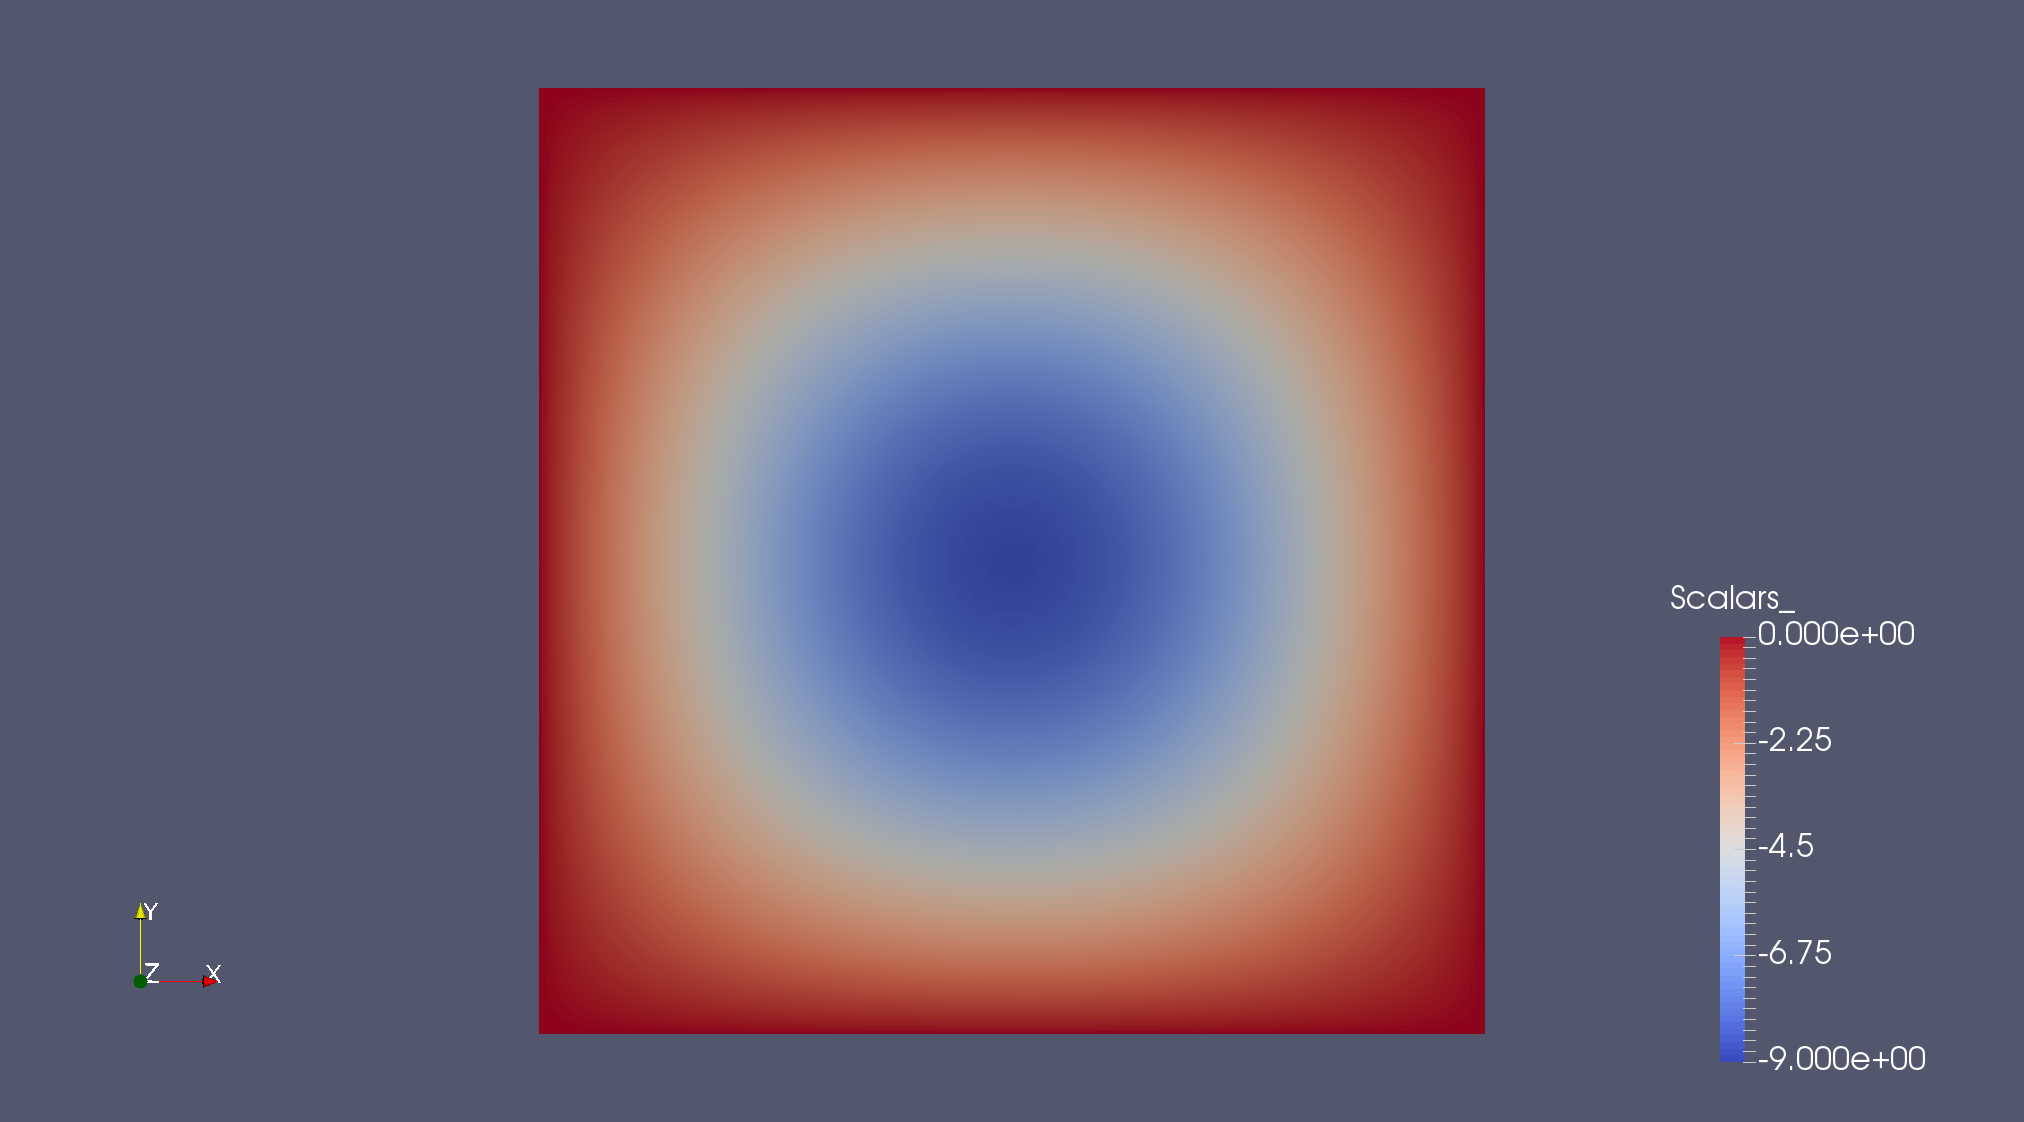
\includegraphics[width=\textwidth]{Images/symm-3r-y-0t.png}
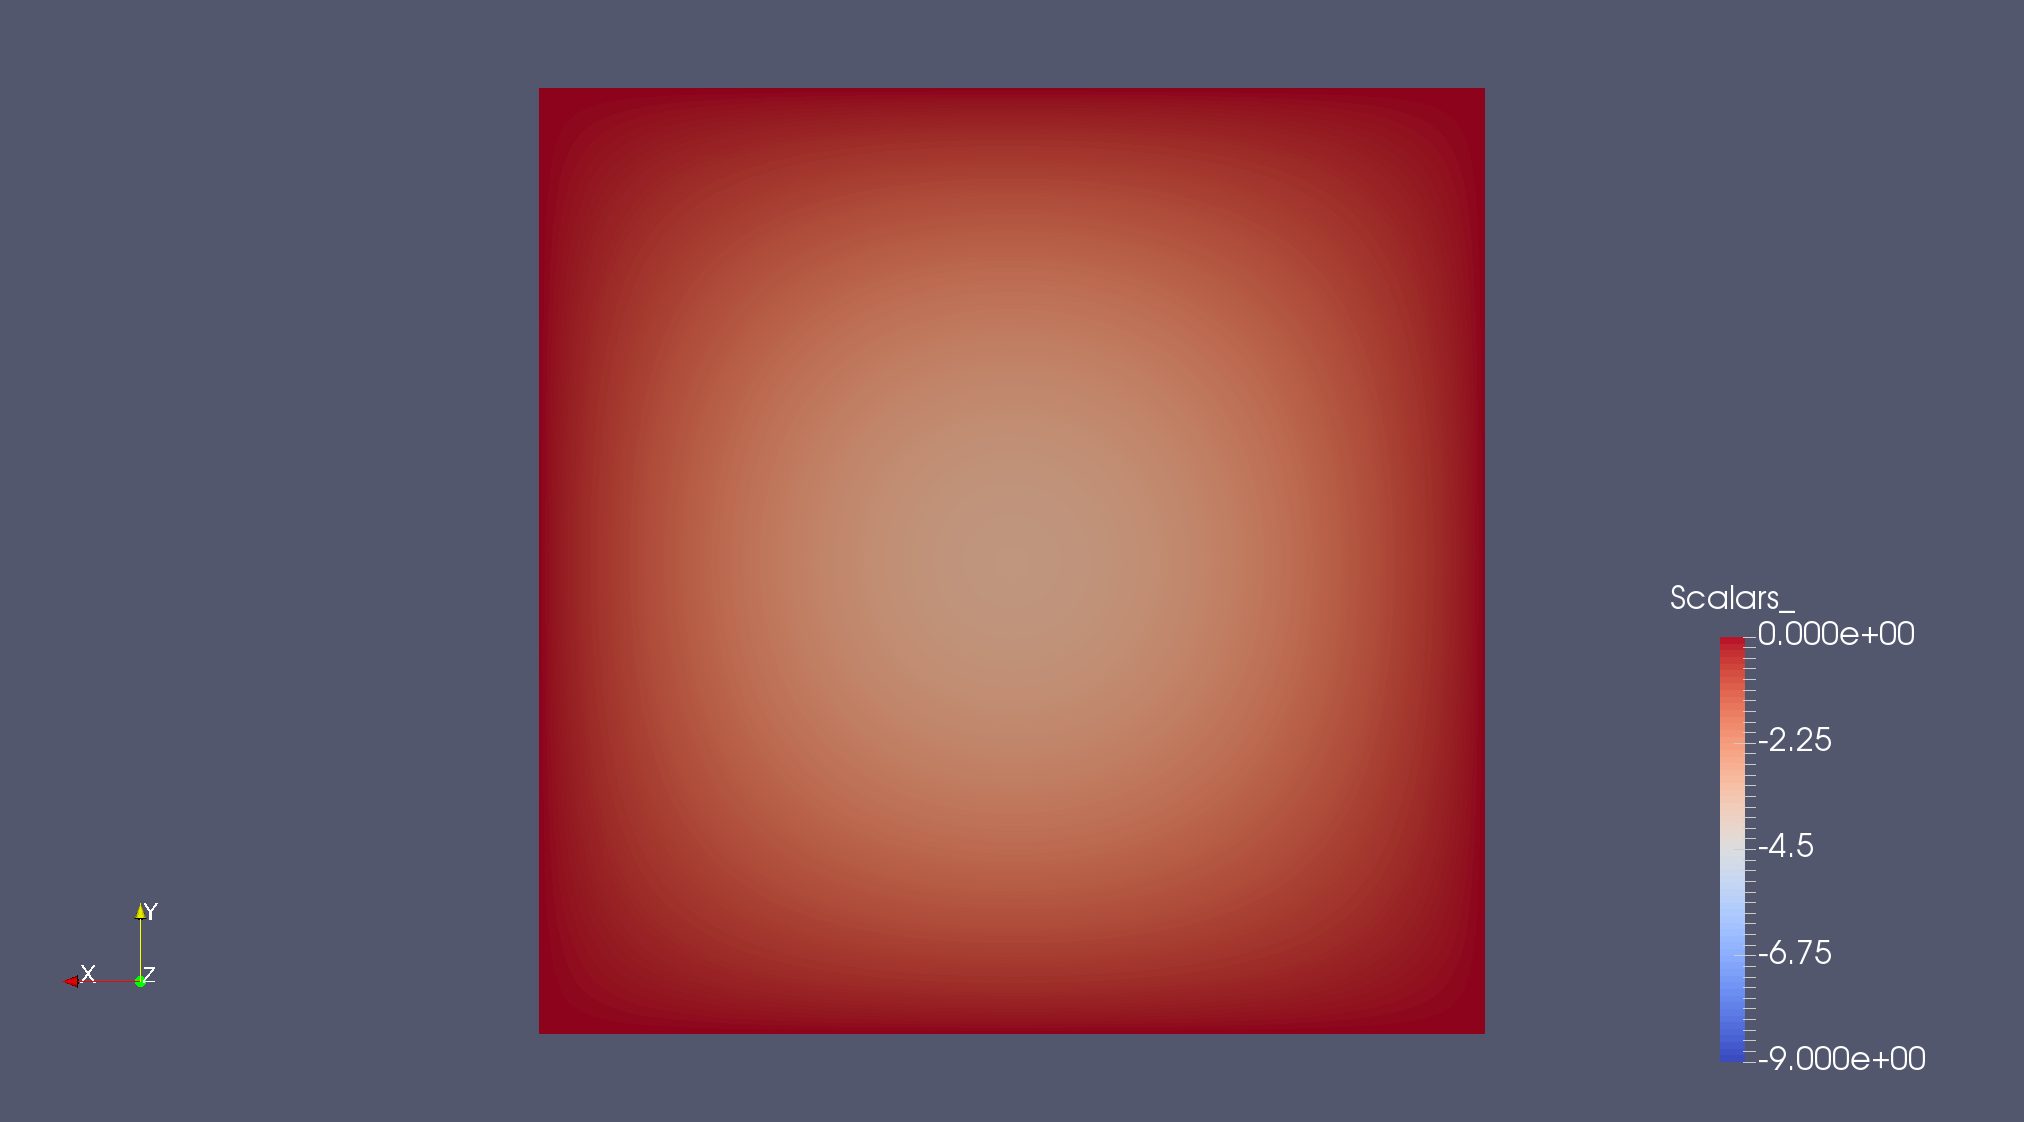
\includegraphics[width=\textwidth]{Images/symm-3r-y-Tt.png}
\caption{The optimal state of the problem \cref{eq:symmetric-num-eq} after 3 times uniform discretization with linear basis functions, at $t = 0$ and $t = T$, respectively.}
\label{fig:symm-3r-y}
\end{figure}
\begin{figure}[htpb]
\centering
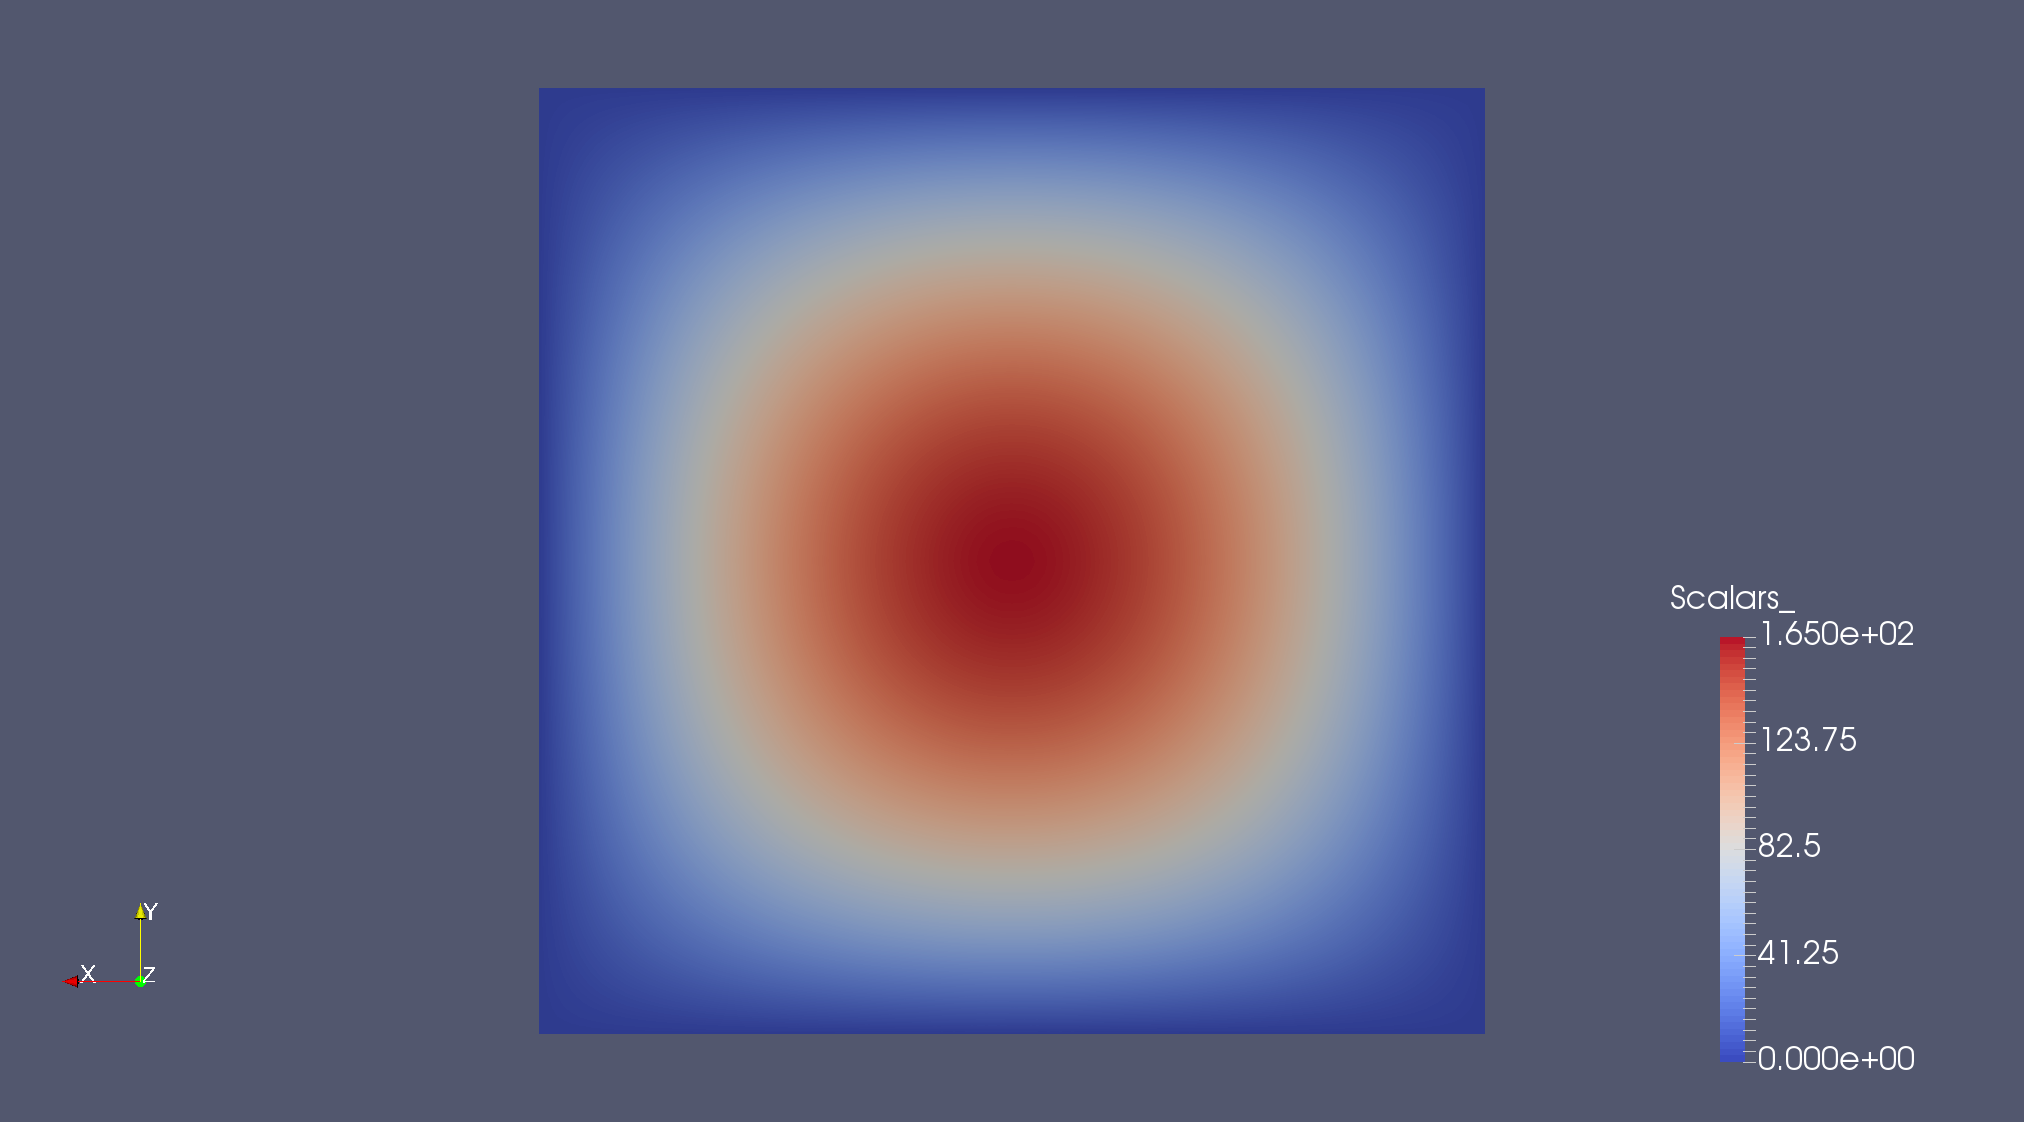
\includegraphics[width=\textwidth]{Images/symm-3r-u-0t.png}
\caption{The optimal control of the problem \cref{eq:symmetric-num-eq} after 3 times uniform discretization with linear basis functions, at $t = 0$. At $t = T$, the control is zero by definition of the optimality system and therefore not shown here.}
\label{fig:symm-3r-u}
\end{figure}
The results in \cref{fig:symm-3r-y,fig:symm-3r-u} were solved using PARDISO by making use of the symmetric matrix formulation we gave in \cref{sec:num-unconstrained}.
\FloatBarrier
Next, we will turn towards the boundary optimal control problem discussed in \cref{sec:boundary-control-opt} and compare results in the unconstrained case and in the case that box restrictions for the control are being made.
Let $\Omega = [0, 1]^2$ and $T = 1$. Moreover, we fix the choices of $\alpha = 1$, $\lambda = 0.1$ and $\beta = 1$.
We will work with quadratic bases now.
Our problem setup shall now be $y_0 \equiv 1$ and $y_\Omega \equiv 40$.
As one would expect, all four sides of the space-time cylinder $Q$ that $u$ works on have the same solution under this setup.
\begin{figure}[htpb]
\centering
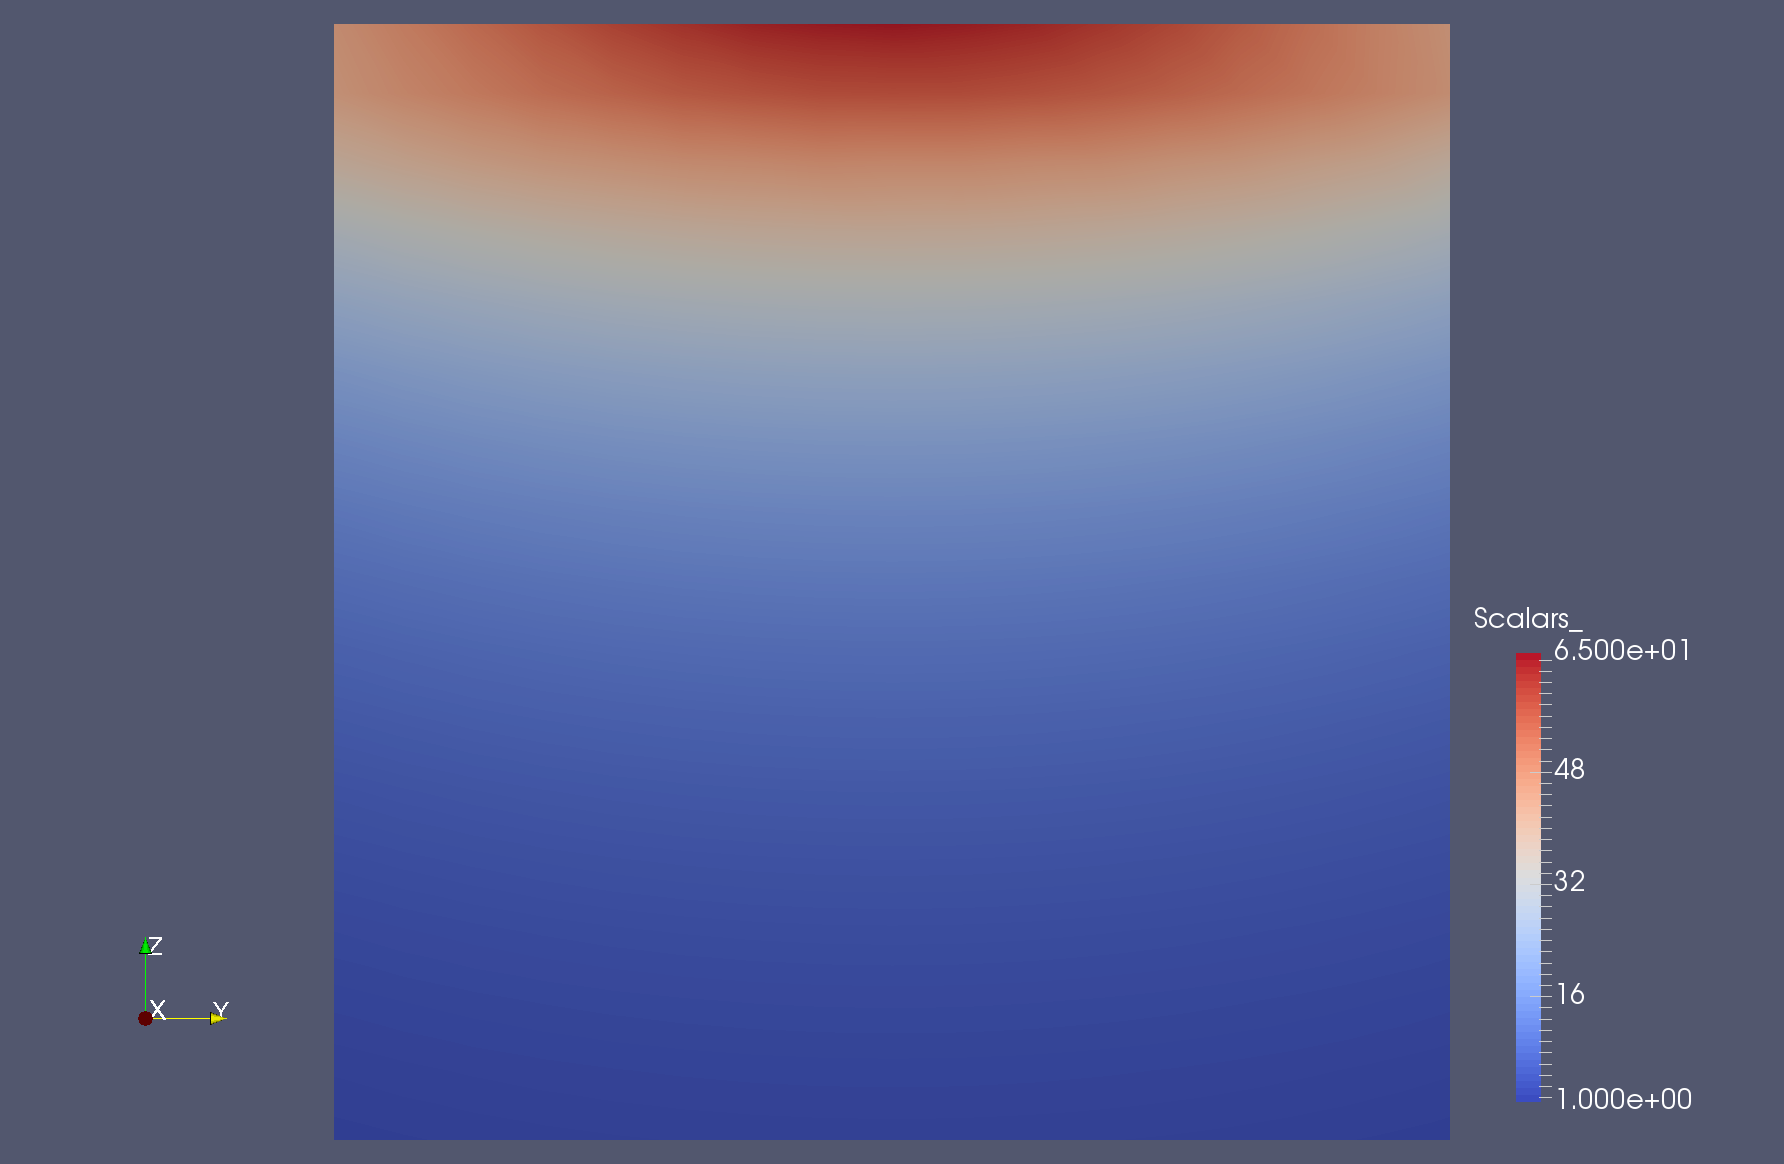
\includegraphics[width=0.9\textwidth]{Images/boundary-const-u.png}
\caption{The optimal control of the boundary control problem with $y_0 \equiv 1$ and $y_\Omega \equiv 40$, plotted at $\{ 1 \} \times [0, 1] \times [0, T]$.}
\label{fig:boundary-const-u}
\end{figure}
As one might expect from the fact that the control in \cref{fig:boundary-const-u} unfolds most of its energy very late on, the state changes very little until shortly before $t = T$. The reason for this is that we effectively made the thermal diffusivity mentioned in \cref{sec:OptimalControlProblem} very large corresponding to a material with physically unreasonable thermal conductivity properties.
This also means that the difference in heat from the boundary towards the center of $\Omega$ is comparatively small.
The \cref{fig:boundary-const-y-endtime} shows the state at the time point $t = T$.

Note that the optimal state does not converge towards $y_\Omega$, as we're penalizing energy required and the boundary control cannot lead towards a constant inner temperature. In fact, the center of the domain, is at the end attaining a value of roughly $29$, whereas the boundary attains values between $34$ and $37$.
In \cref{fig:boundary-const-y-cut} the state of the line $\{ 0.5 \} \times [0, 1]$ is being shown over time.
\begin{figure}[htpb]
\centering
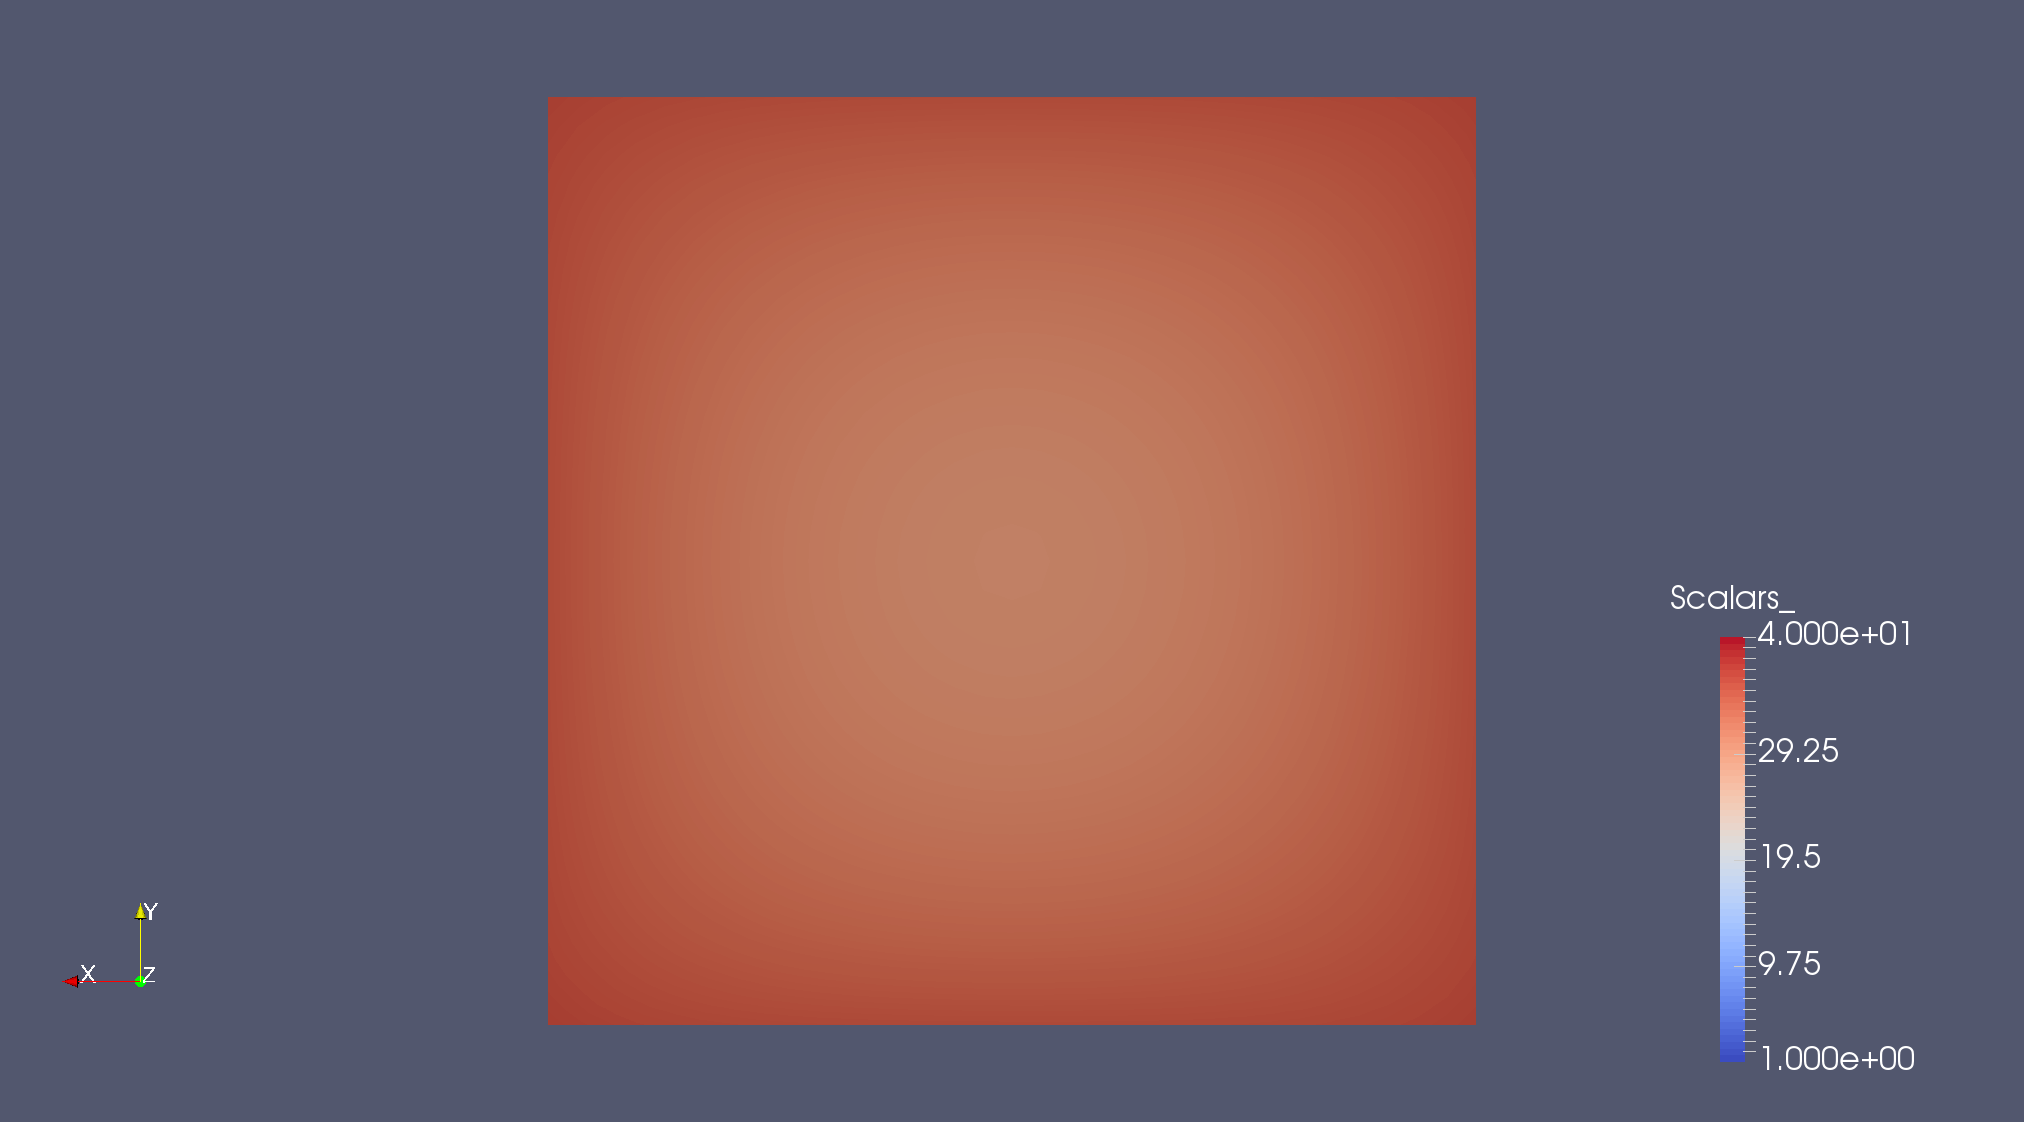
\includegraphics[width=0.9\textwidth]{Images/boundary-const-y-endtime.png}
\caption{The optimal state of the boundary control problem with $y_0 \equiv 1$ and $y_\Omega \equiv 40$, plotted at $t = T$.}
\label{fig:boundary-const-y-endtime}
\end{figure}
\begin{figure}[htpb]
\centering
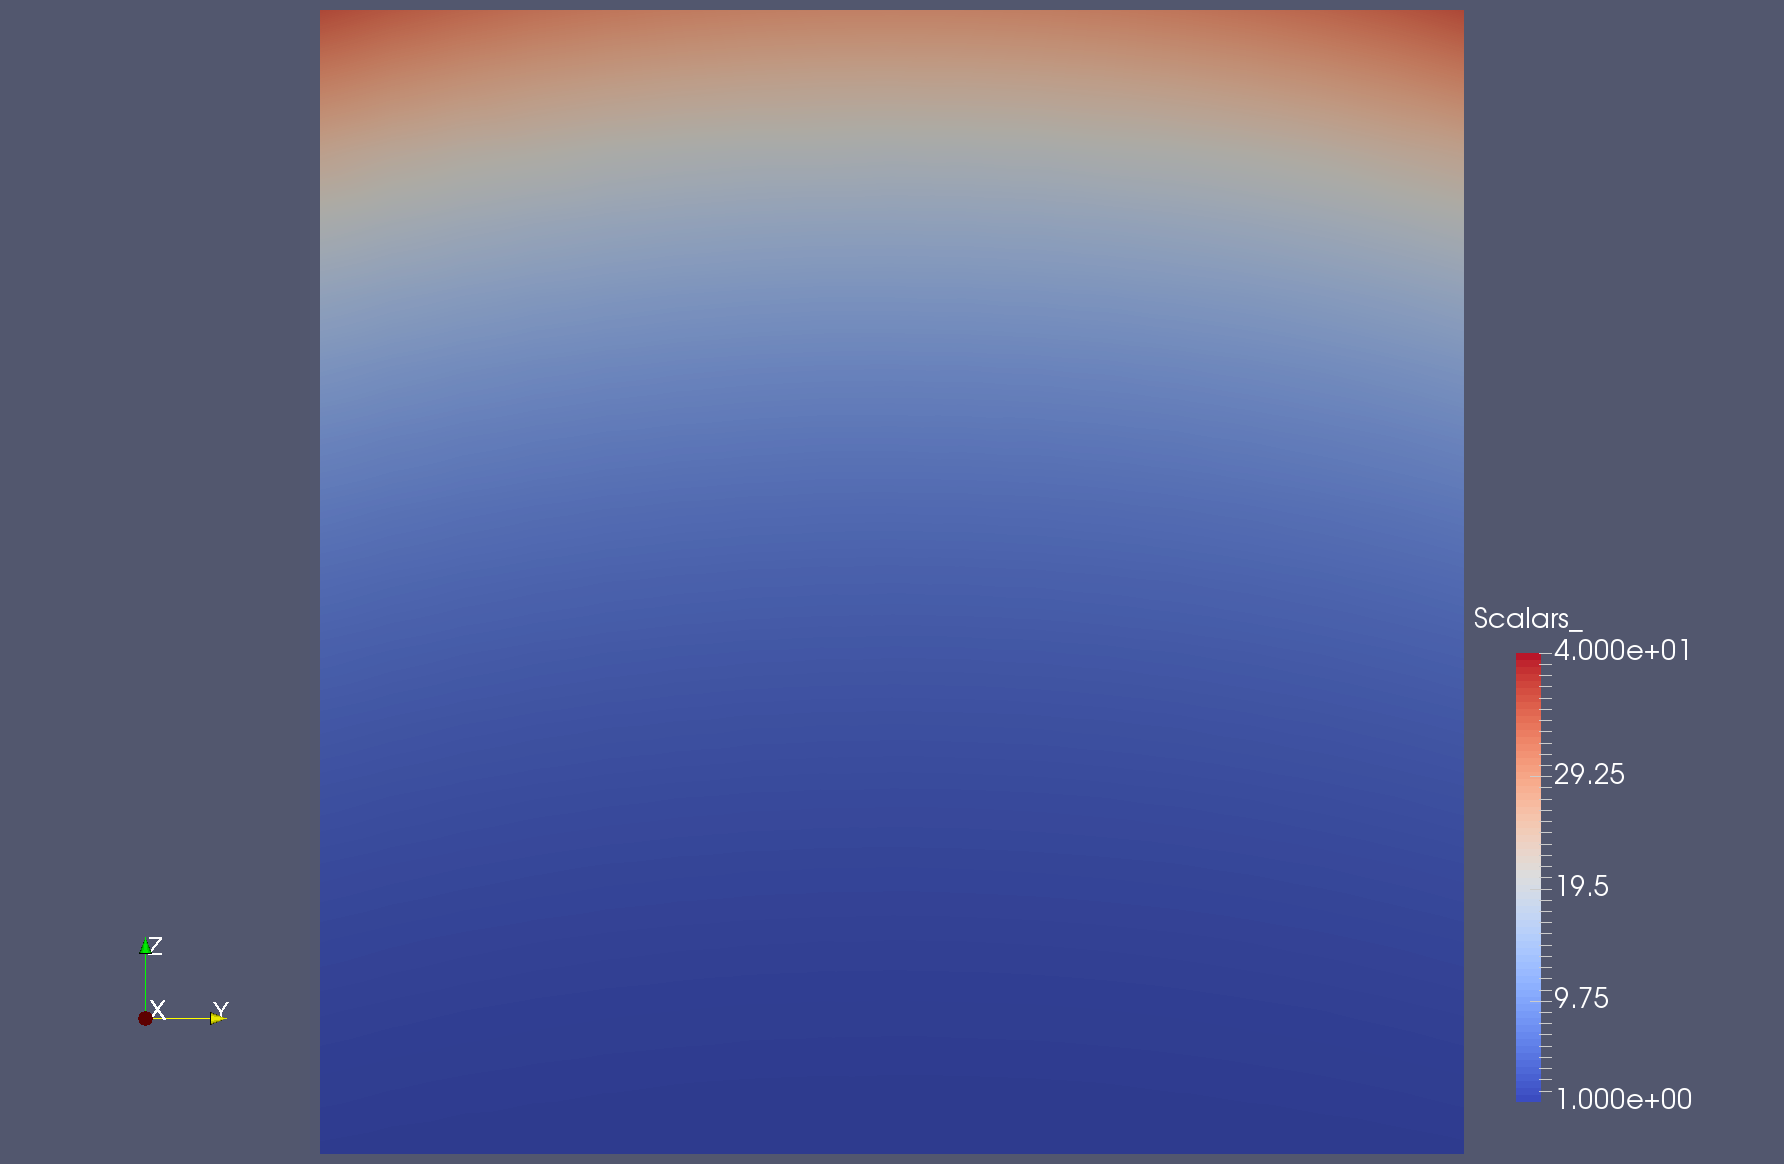
\includegraphics[width=0.9\textwidth]{Images/boundary-const-y-cut.png}
\caption{The optimal state of the boundary control problem with $y_0 \equiv 1$ and $y_\Omega \equiv 40$, plotted as slice $\{ 0.5 \} \times [0, 1] \times [0, 1]$.}
\label{fig:boundary-const-y-cut}
\end{figure}
\FloatBarrier

We can now use the primal-dual active set method described in \cref{sec:KR-numerics} to consider the same problem with the box restrictions $10 \leq u(x, t) \leq 40$. As we've seen, the unrestricted optimal control exceeds these bounds in some points, so the restricted solution should have some cut offs.
The \cref{fig:boundary-const-u-rest} shows the optimal restricted control and \cref{fig:boundary-const-y-rest-endtime} shows its associated state at $t = T$. It took four iterations of the algorithm for it to terminate.
As given by the optimality conditions, one observes that the restricted control is very close to the unrestricted optimal control with a cutoff taking place in the points that exceeds the box constraints.
In fact, the areas where the value $u_a = 10$ and $u_b = 40$ were attained are precisely those that the algorithm placed in $A^-_n$ and $A^+_n$ respectively.

Unlike all other examples discussed in this chapter, these results stem from solving a linear equation system involving a non-symmetric matrix.
The solver PARDISO can handle both, symmetric and non-symmetric matrices alike, but of course it's significantly slower on non-symmetric matrices. Moreover, the amount of memory consumed is roughly doubled.
Therefore, the results for this case step from a three times uniform refinement only, whereas all other results for the boundary and inner optimal control problems in this chapter have at least four refinement steps taken.
\begin{figure}[htpb]
\centering
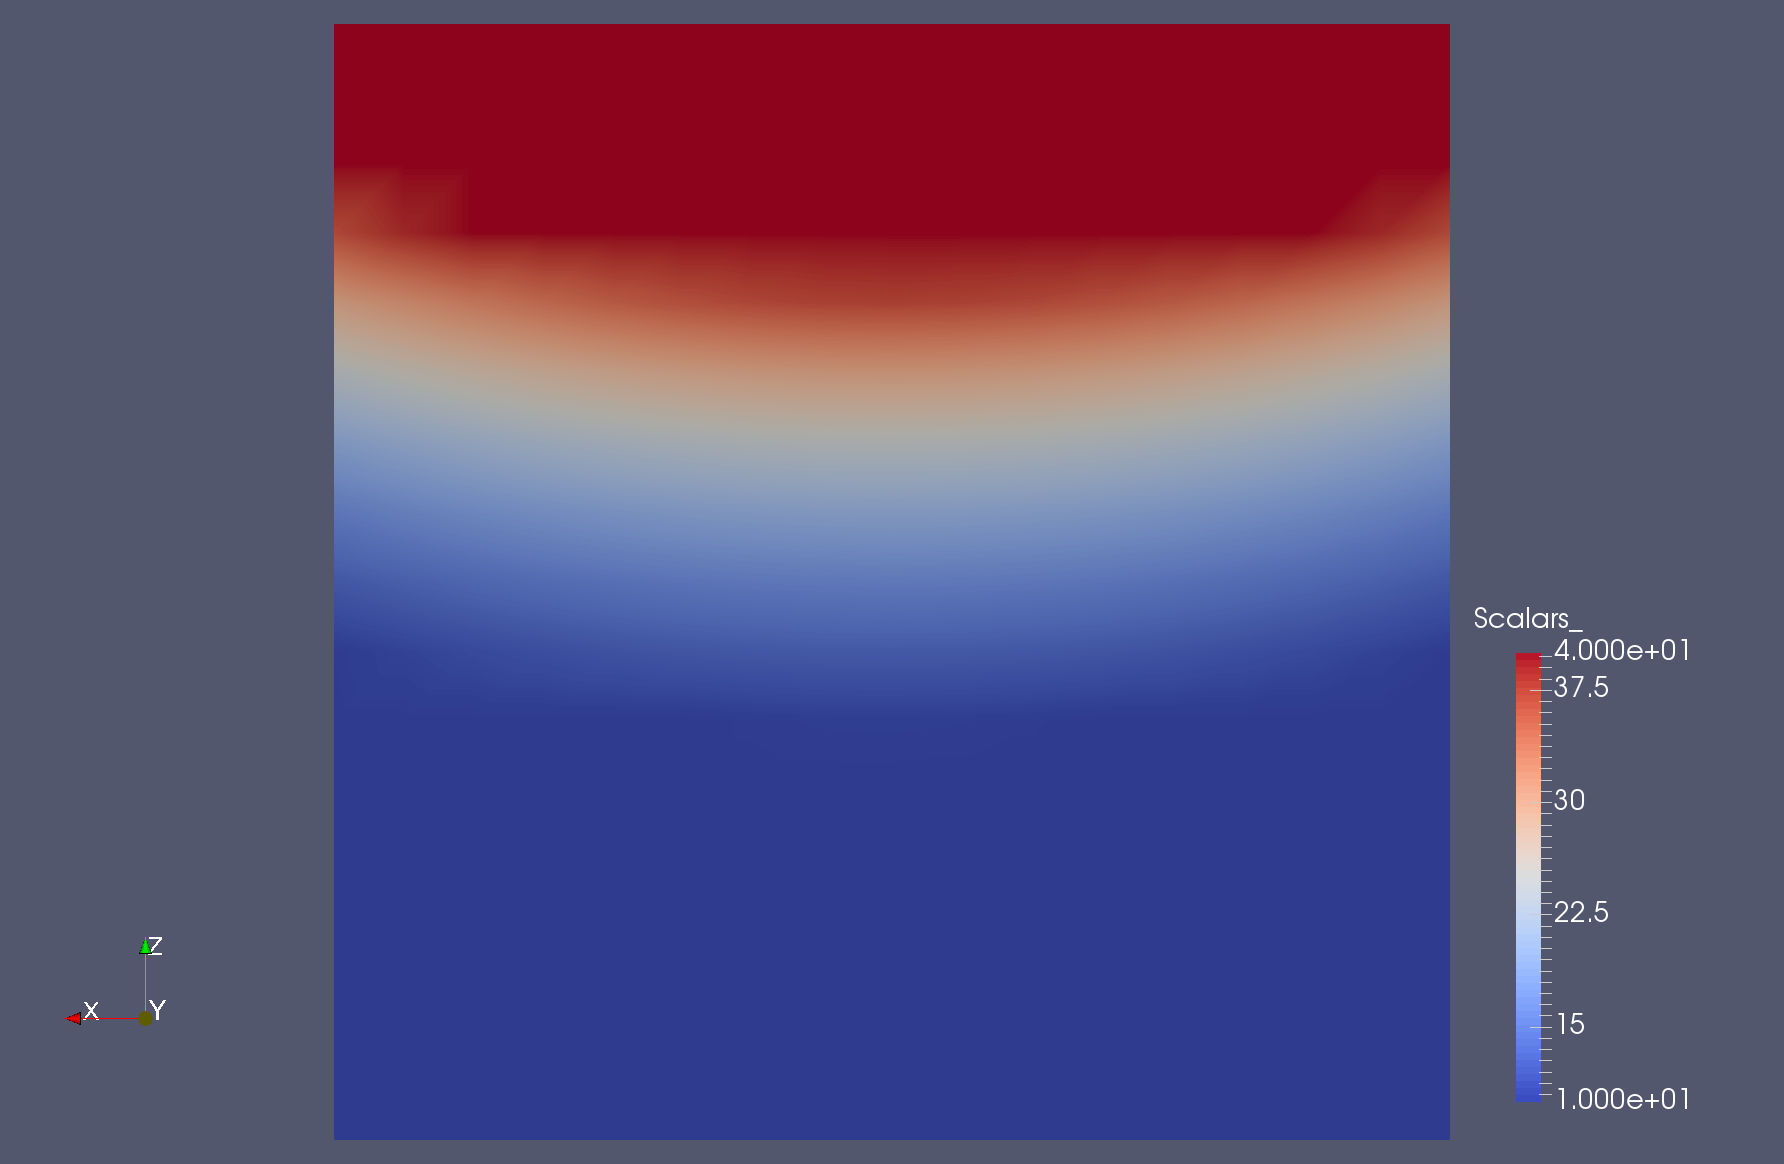
\includegraphics[width=0.9\textwidth]{Images/boundary-cont-u-rest.png}
\caption{The optimal control of the boundary control problem with $y_0 \equiv 1$ and $y_\Omega \equiv 40$ restricted by $10 \leq u(x, t) \leq 40$, plotted at the boundary on $[0, 1] \times \{ 1 \} \times [0, 1]$.}
\label{fig:boundary-const-u-rest}
\end{figure}
\begin{figure}[htpb]
\centering
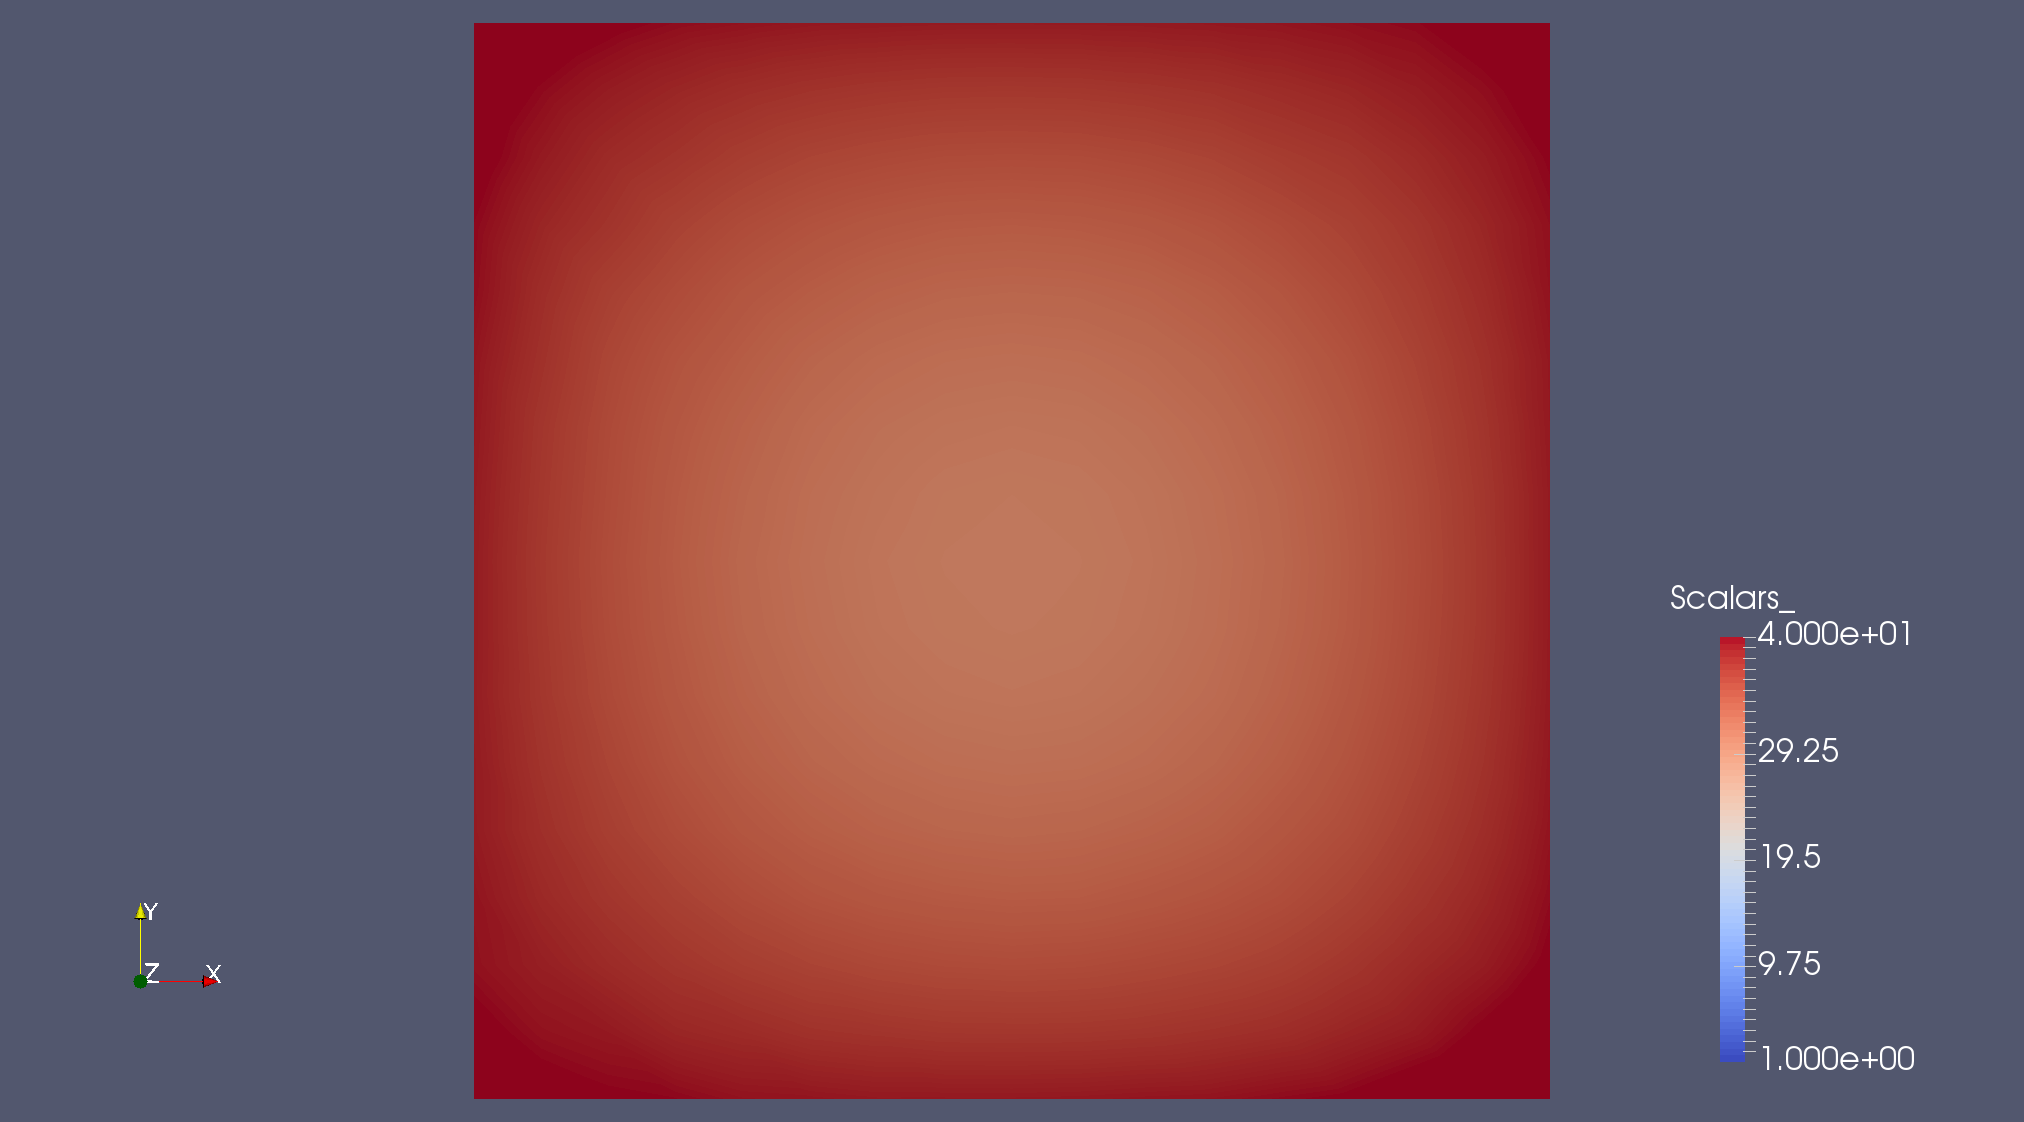
\includegraphics[width=0.9\textwidth]{Images/boundary-cont-y-rest.png}
\caption{The optimal state of the boundary control problem with $y_0 \equiv 1$ and $y_\Omega \equiv 40$ restricted by $10 \leq u(x, t) \leq 40$, plotted at $t = T$.}
\label{fig:boundary-const-y-rest-endtime}
\end{figure}
\FloatBarrier

As previously mentioned, the correct formulation for the heat transfer would be $\partial_t y - \alpha \lapl y = 0$ with the boundary condition $\partial_\nu y + \alpha y = \alpha u$.
Numerically, a coefficient in front of the Laplace term will cause stability issues if it gets too small.
As far as the theory is concerned, nothing changes except for the term $\alpha$ appearing as coefficient in front of all norms and so forth.
We want to see what changing the coefficient of the Laplace term does to the optimal control.
Therefore, we now pick $\alpha = 0.2$ for all three occurrences. Other than that, we leave the problem setup unchanged.
We have displayed one side of the control in \cref{fig:boundary-lowthet-u} and the associated states as before in \cref{fig:boundary-lowthet-y-endtime,fig:boundary-lowthet-y-cut}.
In order to improve the readability, we have set the upper limit of the color scale to $30$ in these figures, whereas $y_\Omega \equiv 40$.
One notices right away that the state is being heated up much earlier in time than before and that the overall state at $t = T$ is much farther away from $y_\Omega$ than it was before.
By changing the value of $\alpha$ on the boundary, or more specifically, the value of $\beta$, the control needs much more energy to attain the same heating effect.
Additionally, the introduction of the parameter $\alpha$ in front of the Laplace term ensures that in order to attain the same end-time state, a control has to heat up earlier as the transport of heat inside the domain $\Omega$ is not as good anymore.
\begin{figure}[htpb]
\centering
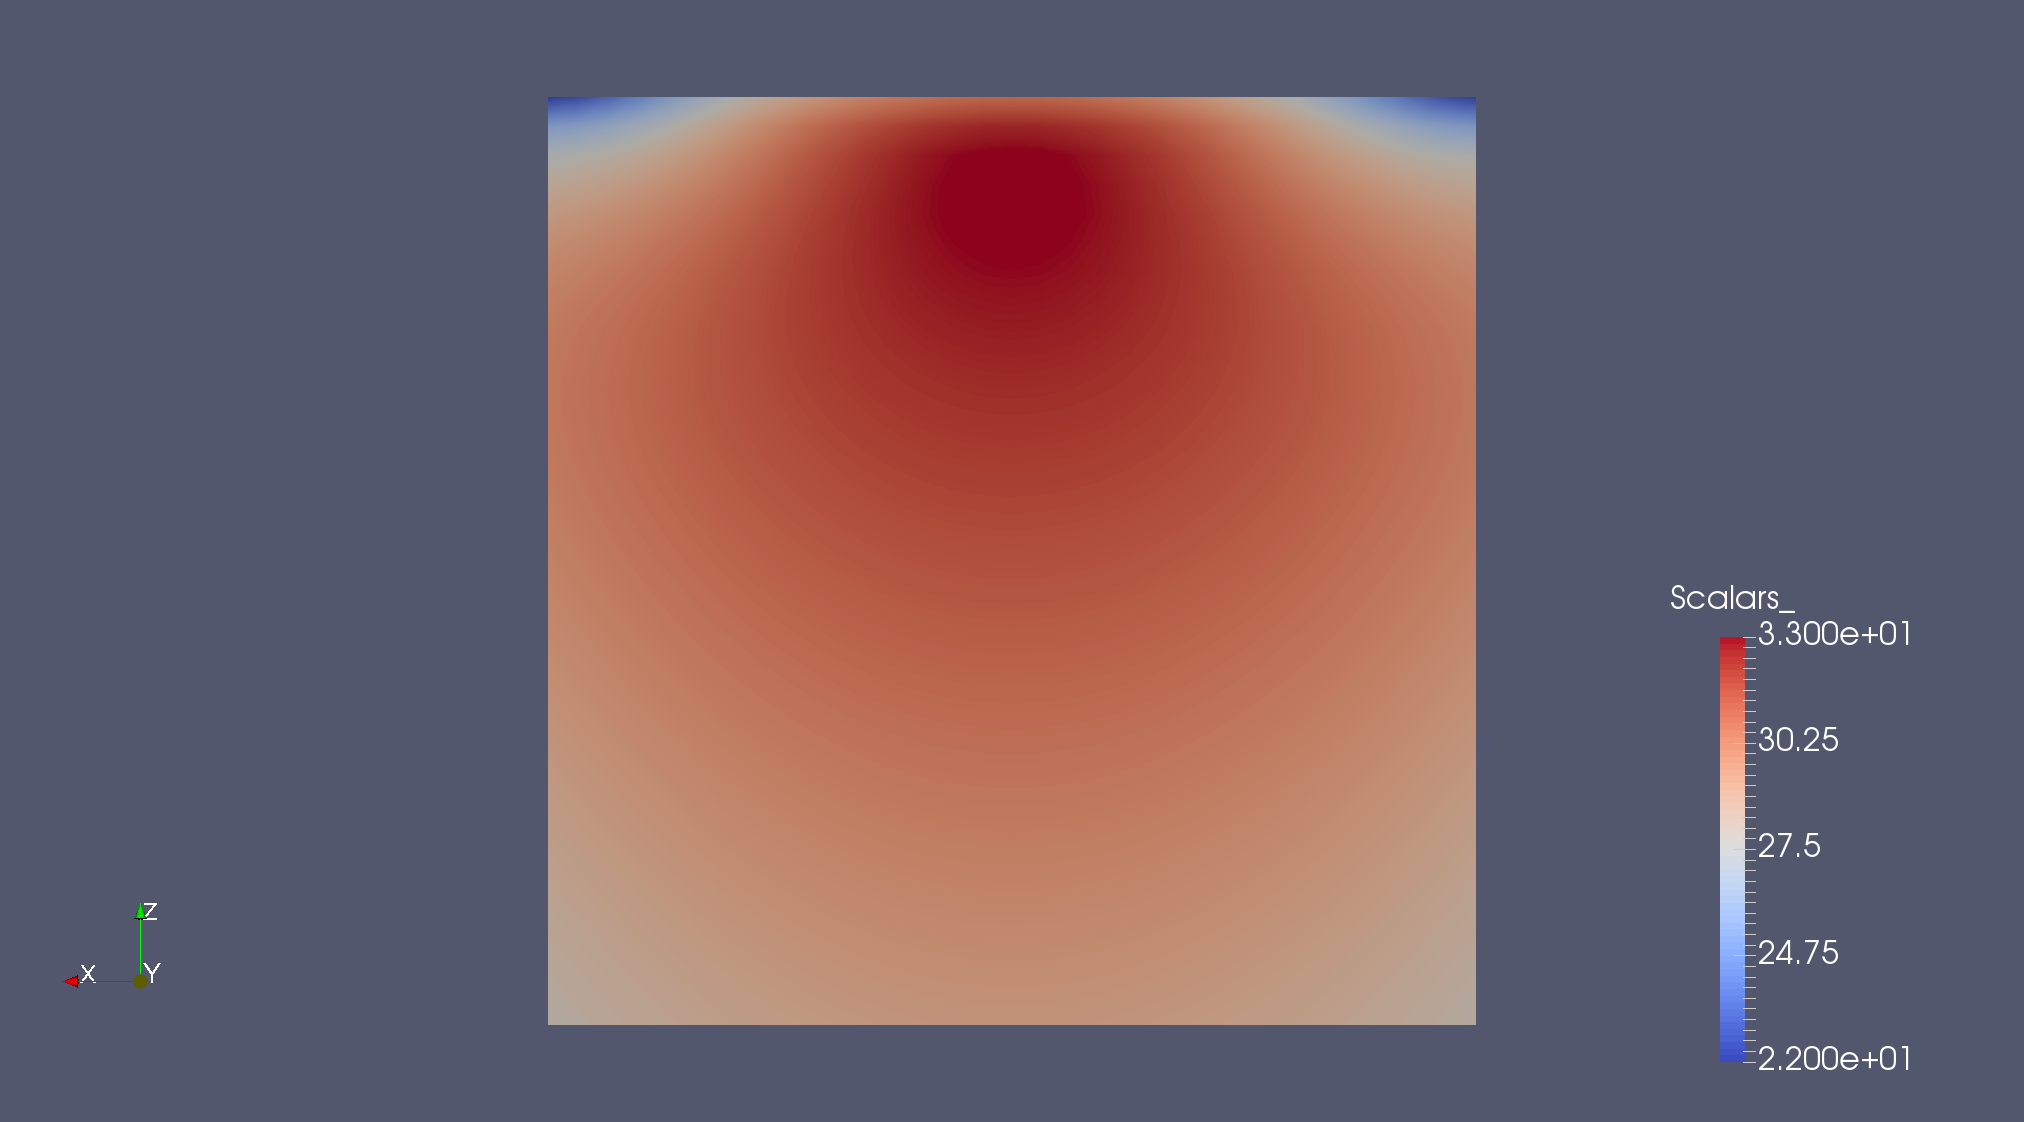
\includegraphics[width=\textwidth]{Images/boundary-lowthet-u.png}
\caption{The optimal control of the boundary control problem with $y_0 \equiv 1$ and $y_\Omega \equiv 40$ and $\alpha = 0.2$, plotted at the boundary on $[0, 1] \times \{ 1 \} \times [0, 1]$.}
\label{fig:boundary-lowthet-u}
\end{figure}
\begin{figure}[htpb]
\centering
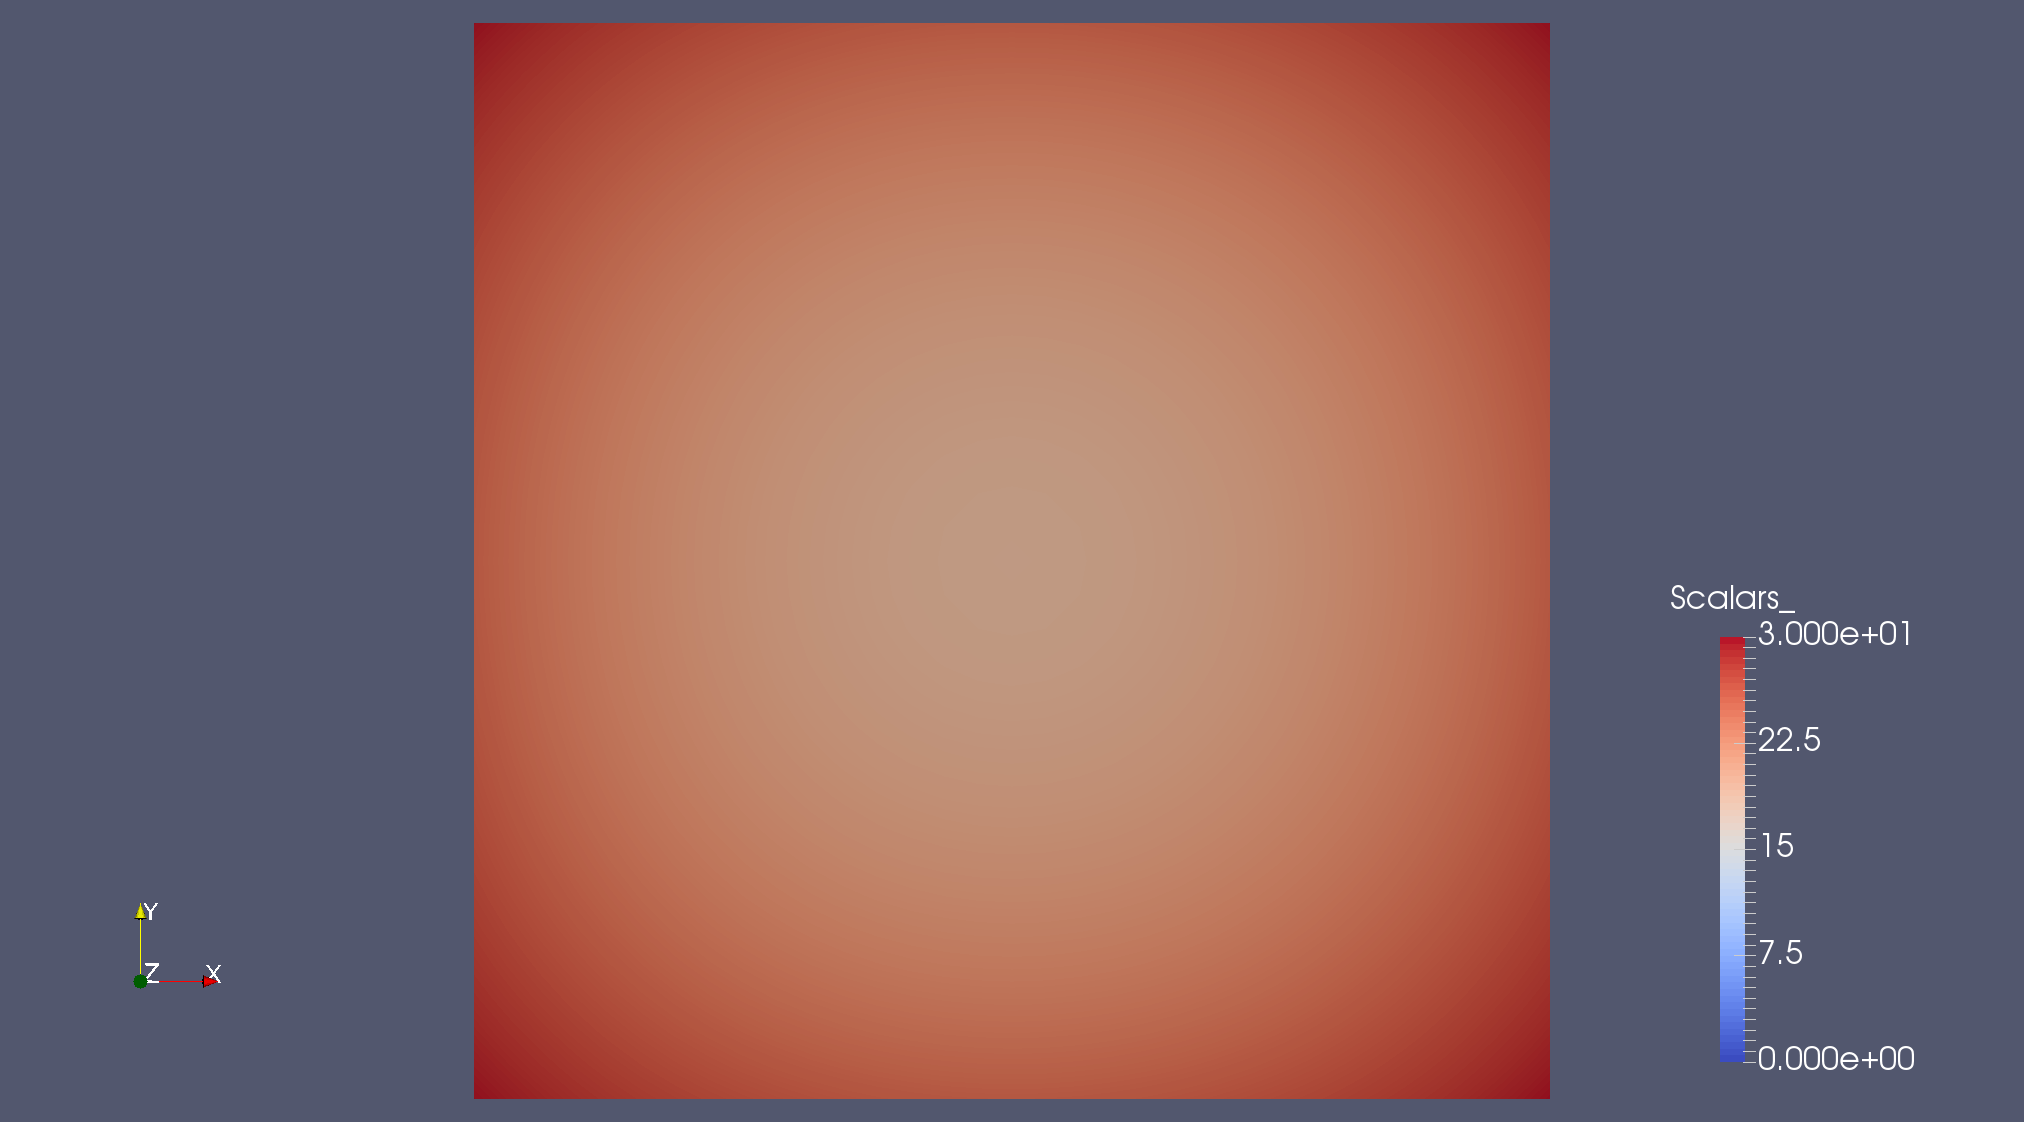
\includegraphics[width=\textwidth]{Images/boundary-lowthet-y-endtime.png}
\caption{The optimal state of the boundary control problem with $y_0 \equiv 1$ and $y_\Omega \equiv 40$ and $\alpha = 0.2$, plotted at $t = T$.}
\label{fig:boundary-lowthet-y-endtime}
\end{figure}
\begin{figure}[htpb]
\centering
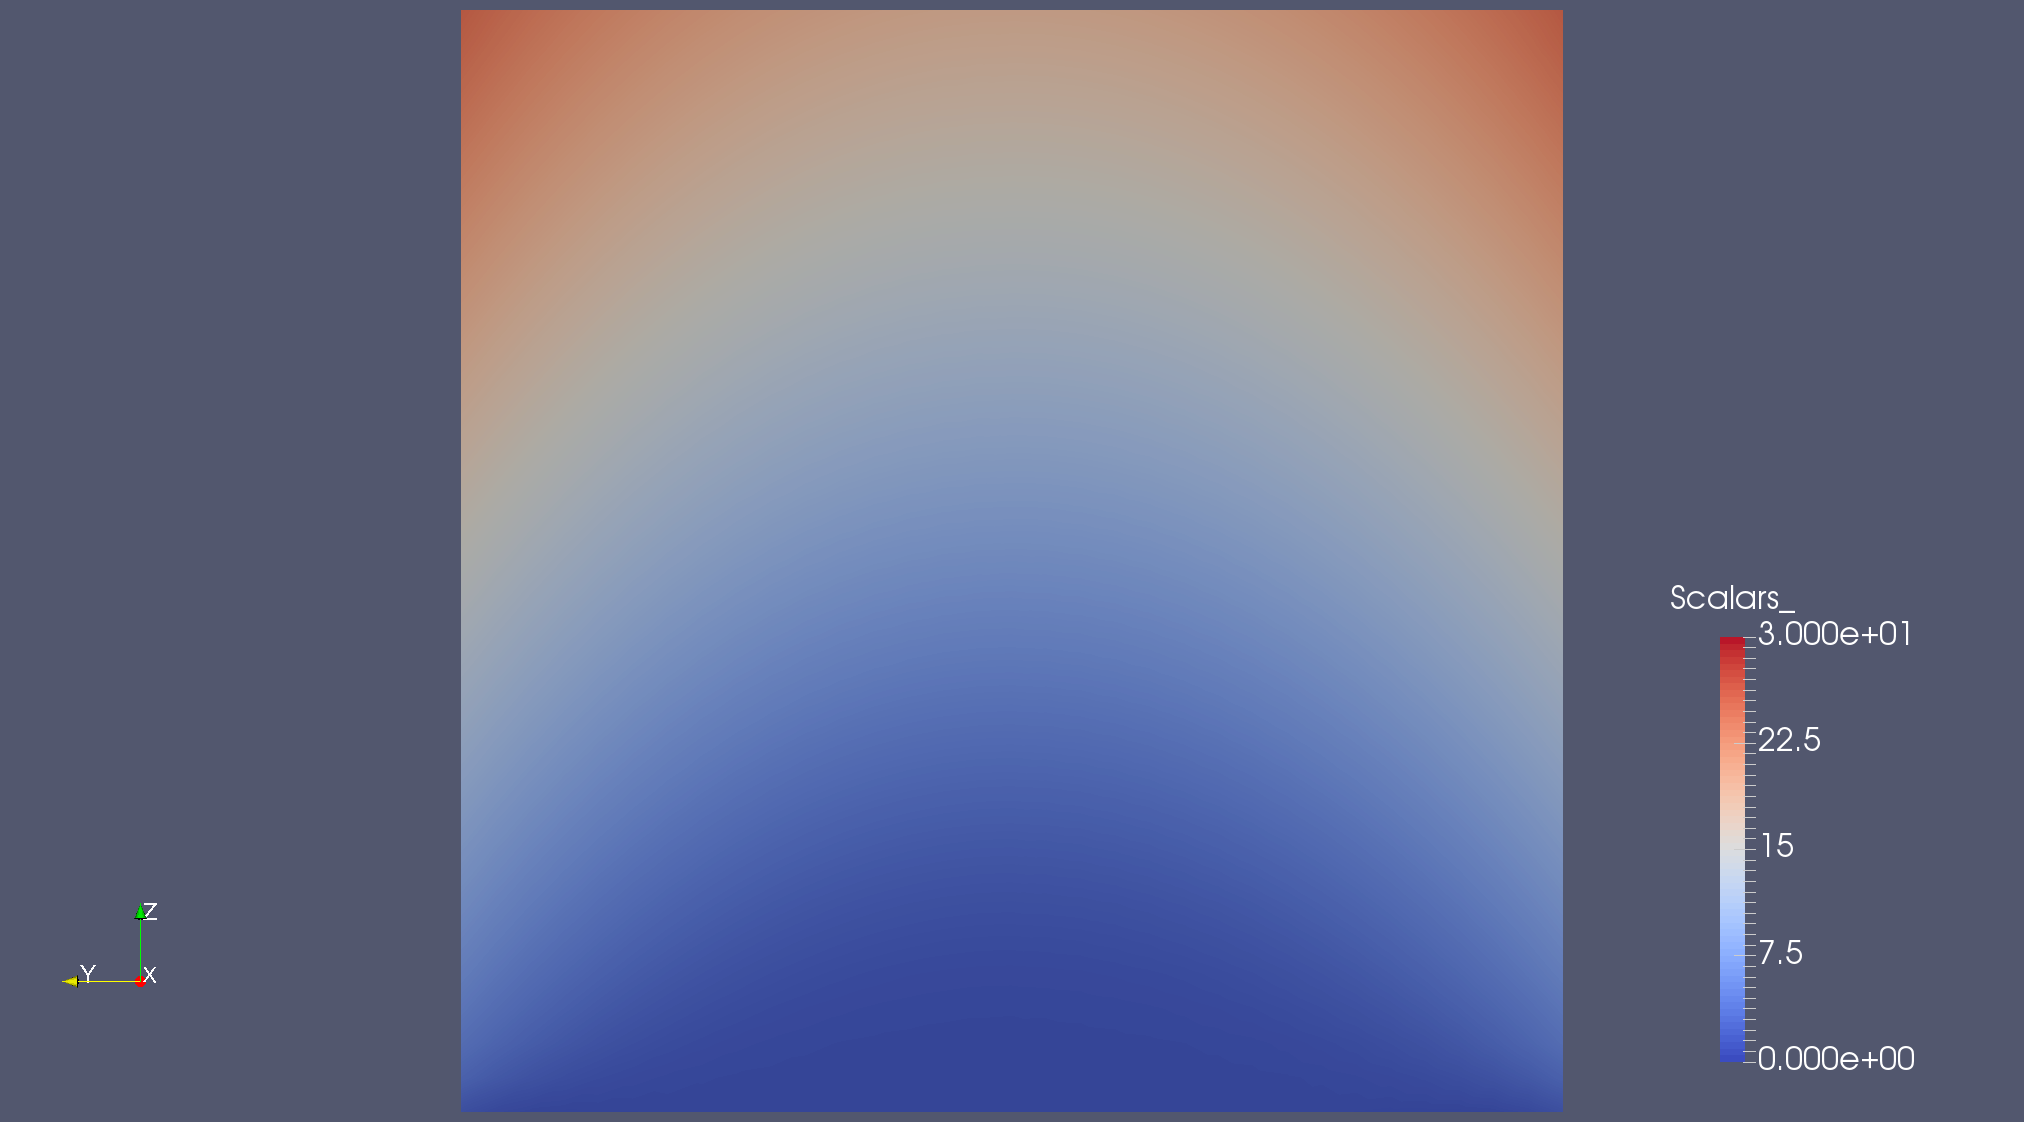
\includegraphics[width=\textwidth]{Images/boundary-lowthet-y-cut.png}
\caption{The optimal state of the boundary control problem with $y_0 \equiv 1$ and $y_\Omega \equiv 40$ and $\alpha = 0.2$, plotted as slice $\{ 0.5 \} \times [0, 1] \times [0, 1]$.}
\label{fig:boundary-lowthet-y-cut}
\end{figure}
\FloatBarrier

Finally, we want to show some results for \cref{sec:inner-optimal-control}.
Let the domain and $\lambda = 0.1$ as before, $\alpha = 0$ and $\beta = 1$. Once again, we use the quadratic basis functions.
For $y_Q$ we will now use a non-constant function:
\[
	y_Q(x, y, t) = (x + y) \sin(\pi t).
\]
As $y_Q$ differs between time points by a scaling factor, we show the results for the optimal state at $t = 0.5$ in \cref{fig:inner-y-midtime}.
Due to the way the state looks, we cut the state for display reasons along the line going from $(0, 0)$ to $(1, 1)$ and displayed the behavior over time in \cref{fig:inner-y-diag}.
\cref{fig:inner-u-midtime,fig:inner-u-diag} show the optimal control cut away in the same fashion.
\begin{figure}[htpb]
\centering
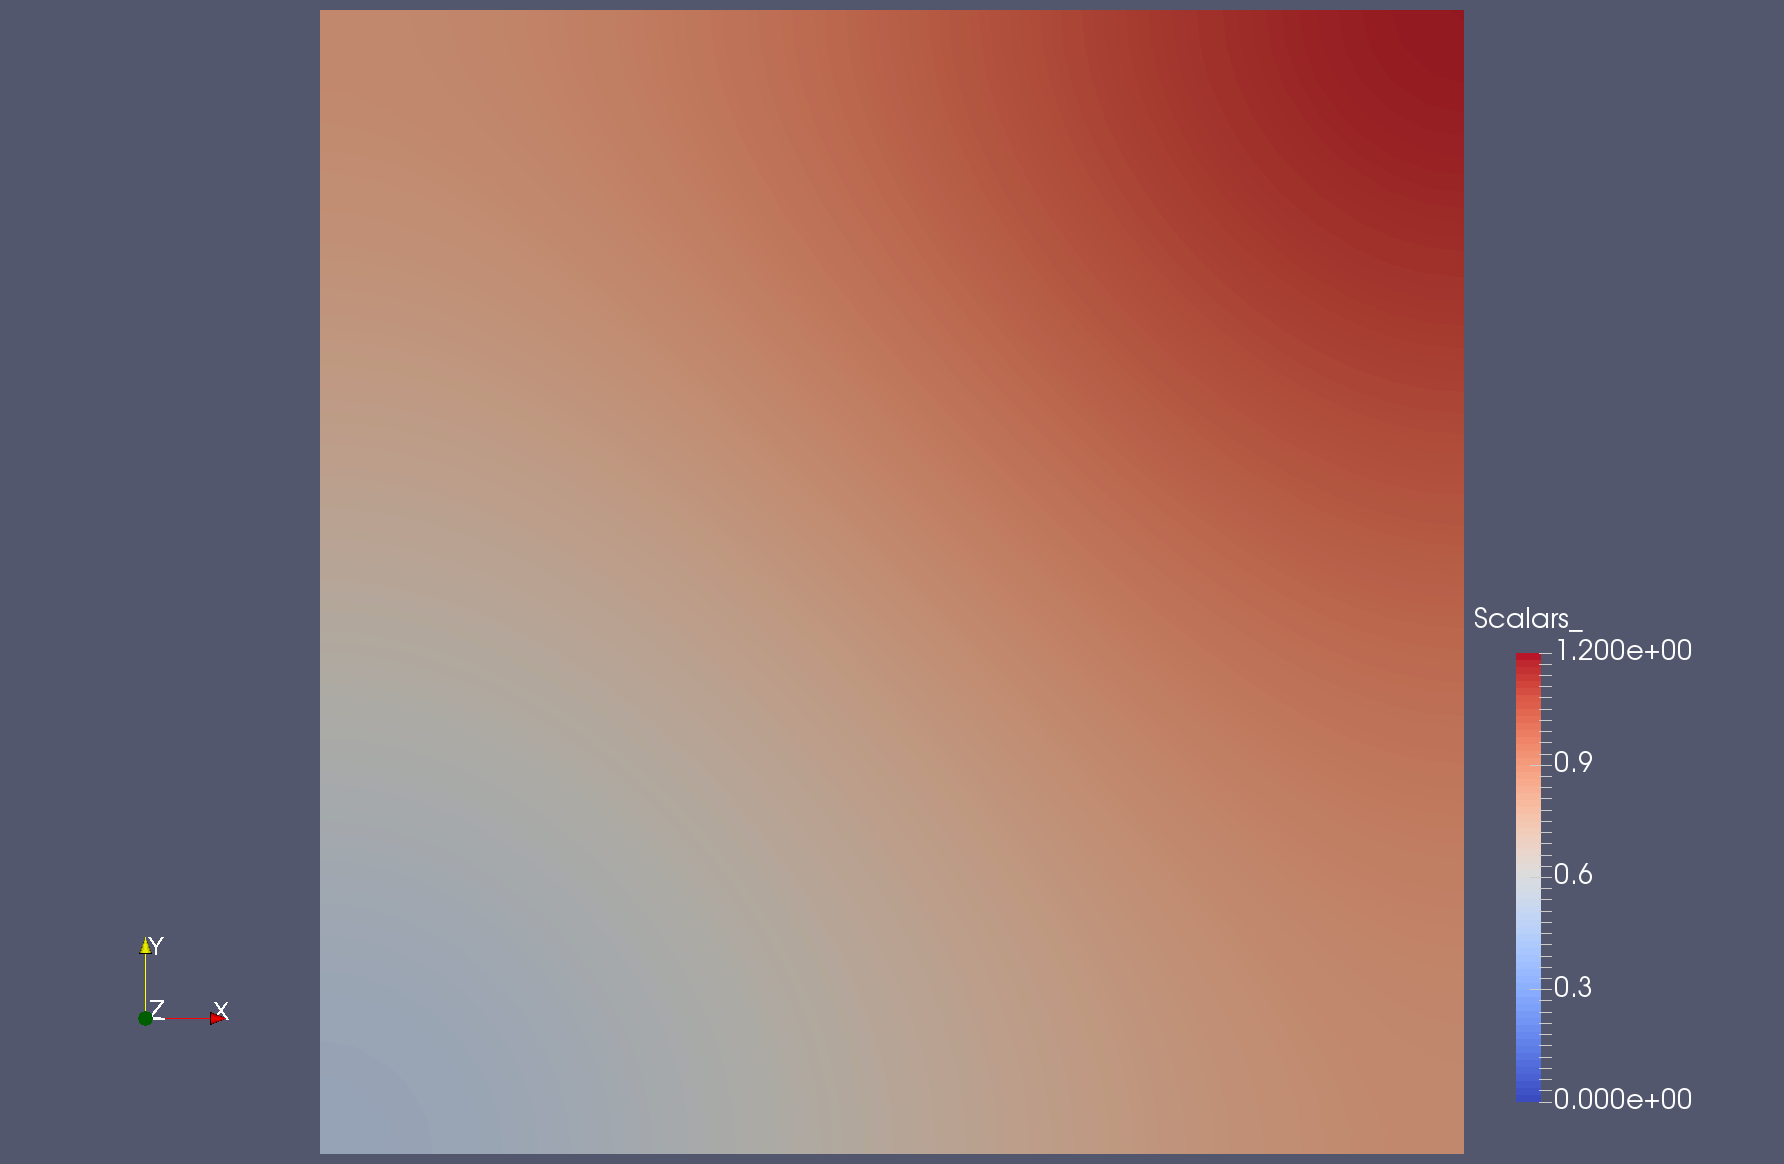
\includegraphics[width=0.9\textwidth]{Images/inner-y-cut-midtime.png}
\caption{The optimal state of the inner control problem, plotted at $t = 0.5$.}
\label{fig:inner-y-midtime}
\end{figure}
\begin{figure}[htpb]
\centering
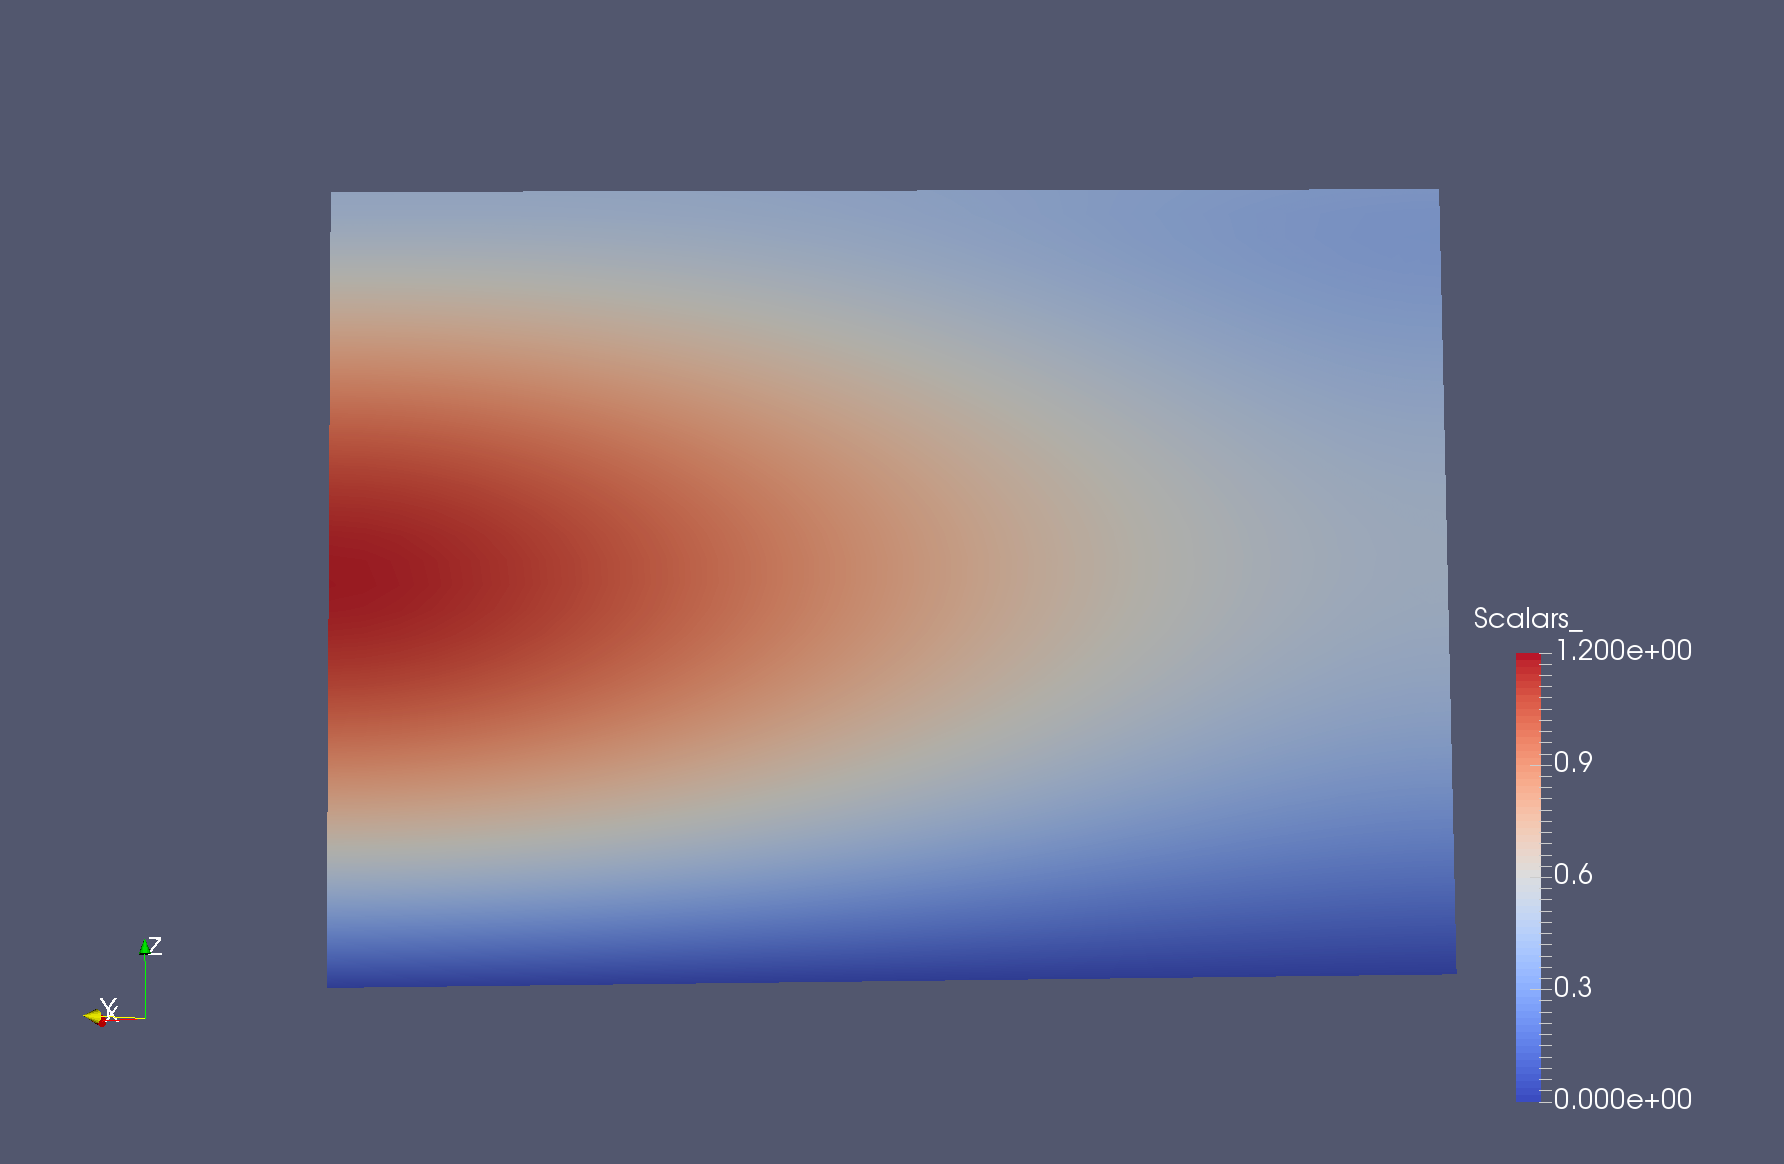
\includegraphics[width=0.9\textwidth]{Images/inner-y-cut-diag.png}
\caption{The optimal state of the inner control problem, plotted as a cut along the diagonal plane with normal $(-1, 1, 0)^\tp$ centered on $(0.5, 0.5, 0.5)^\tp$.}
\label{fig:inner-y-diag}
\end{figure}
\begin{figure}[htpb]
\centering
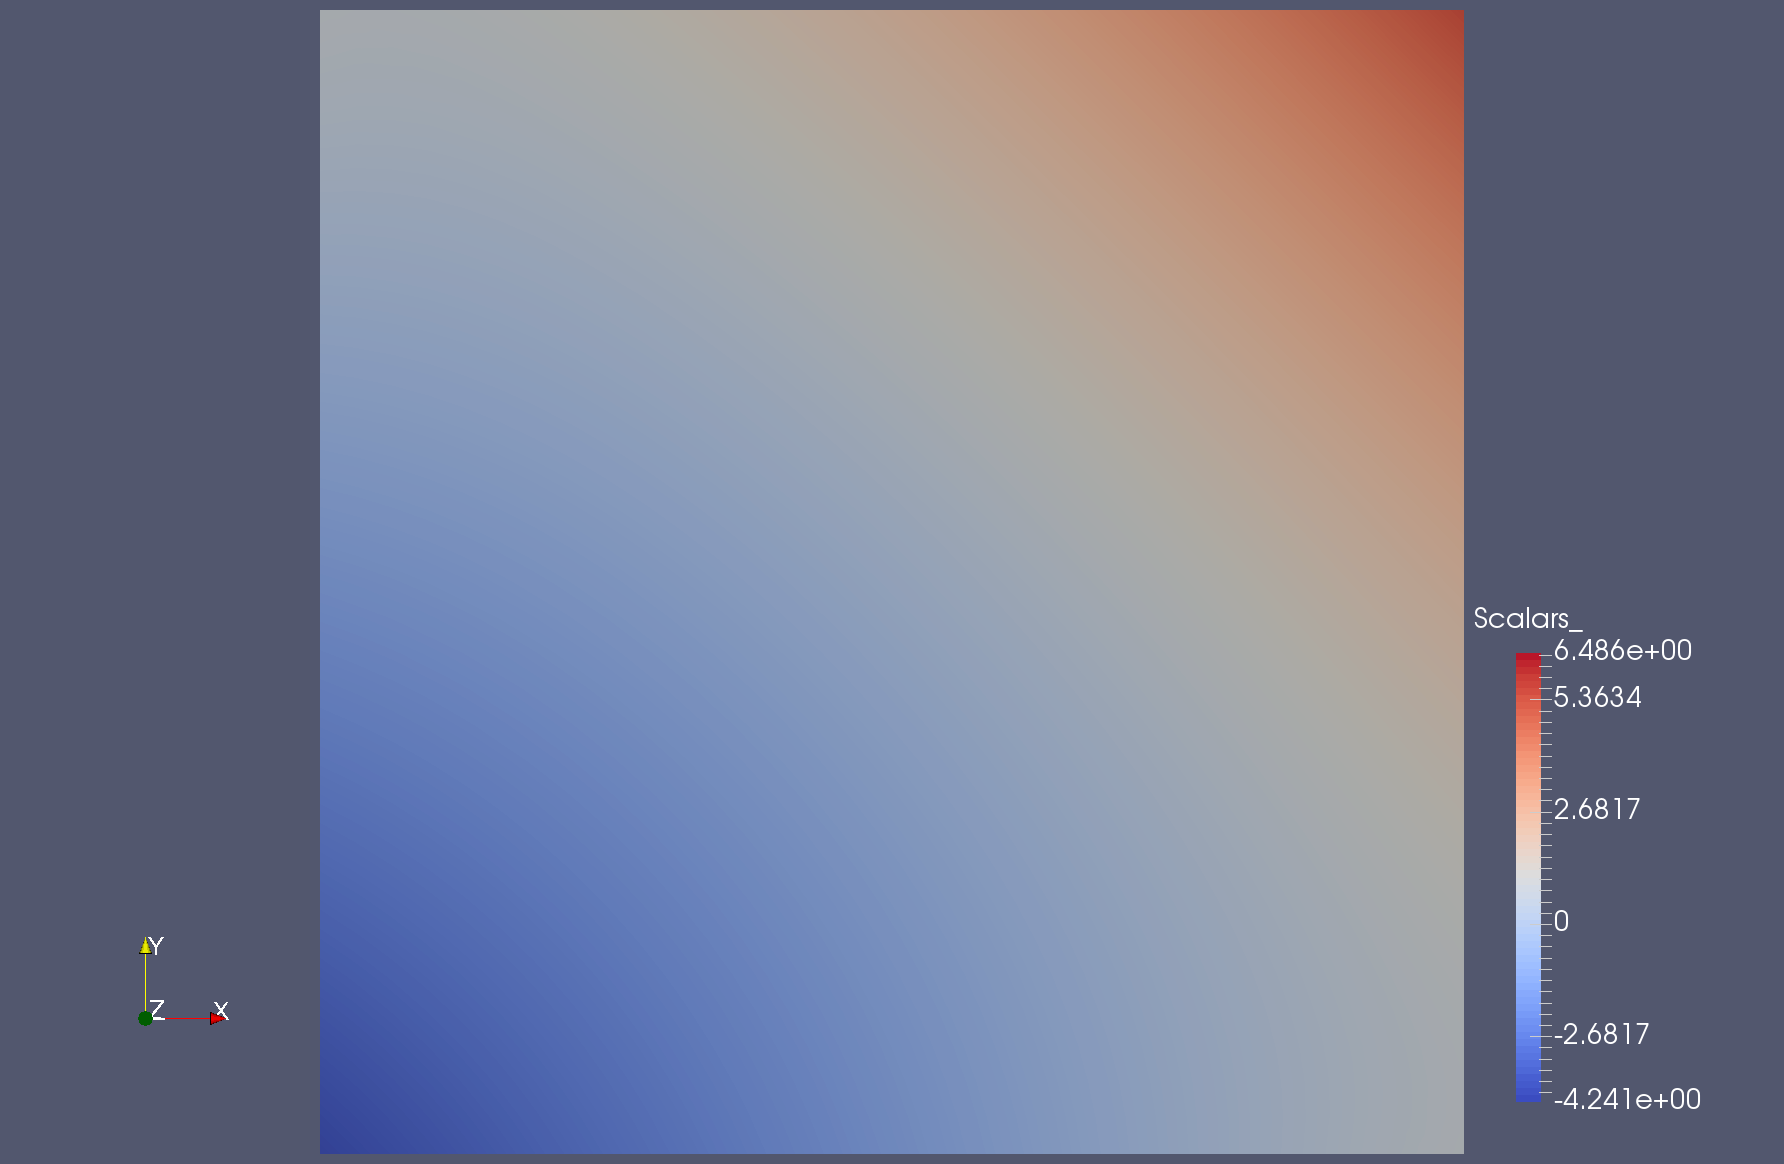
\includegraphics[width=0.9\textwidth]{Images/inner-u-cut-midtime.png}
\caption{The optimal control of the inner control problem, plotted at $t = 0.5$.}
\label{fig:inner-u-midtime}
\end{figure}
\begin{figure}[htpb]
\centering
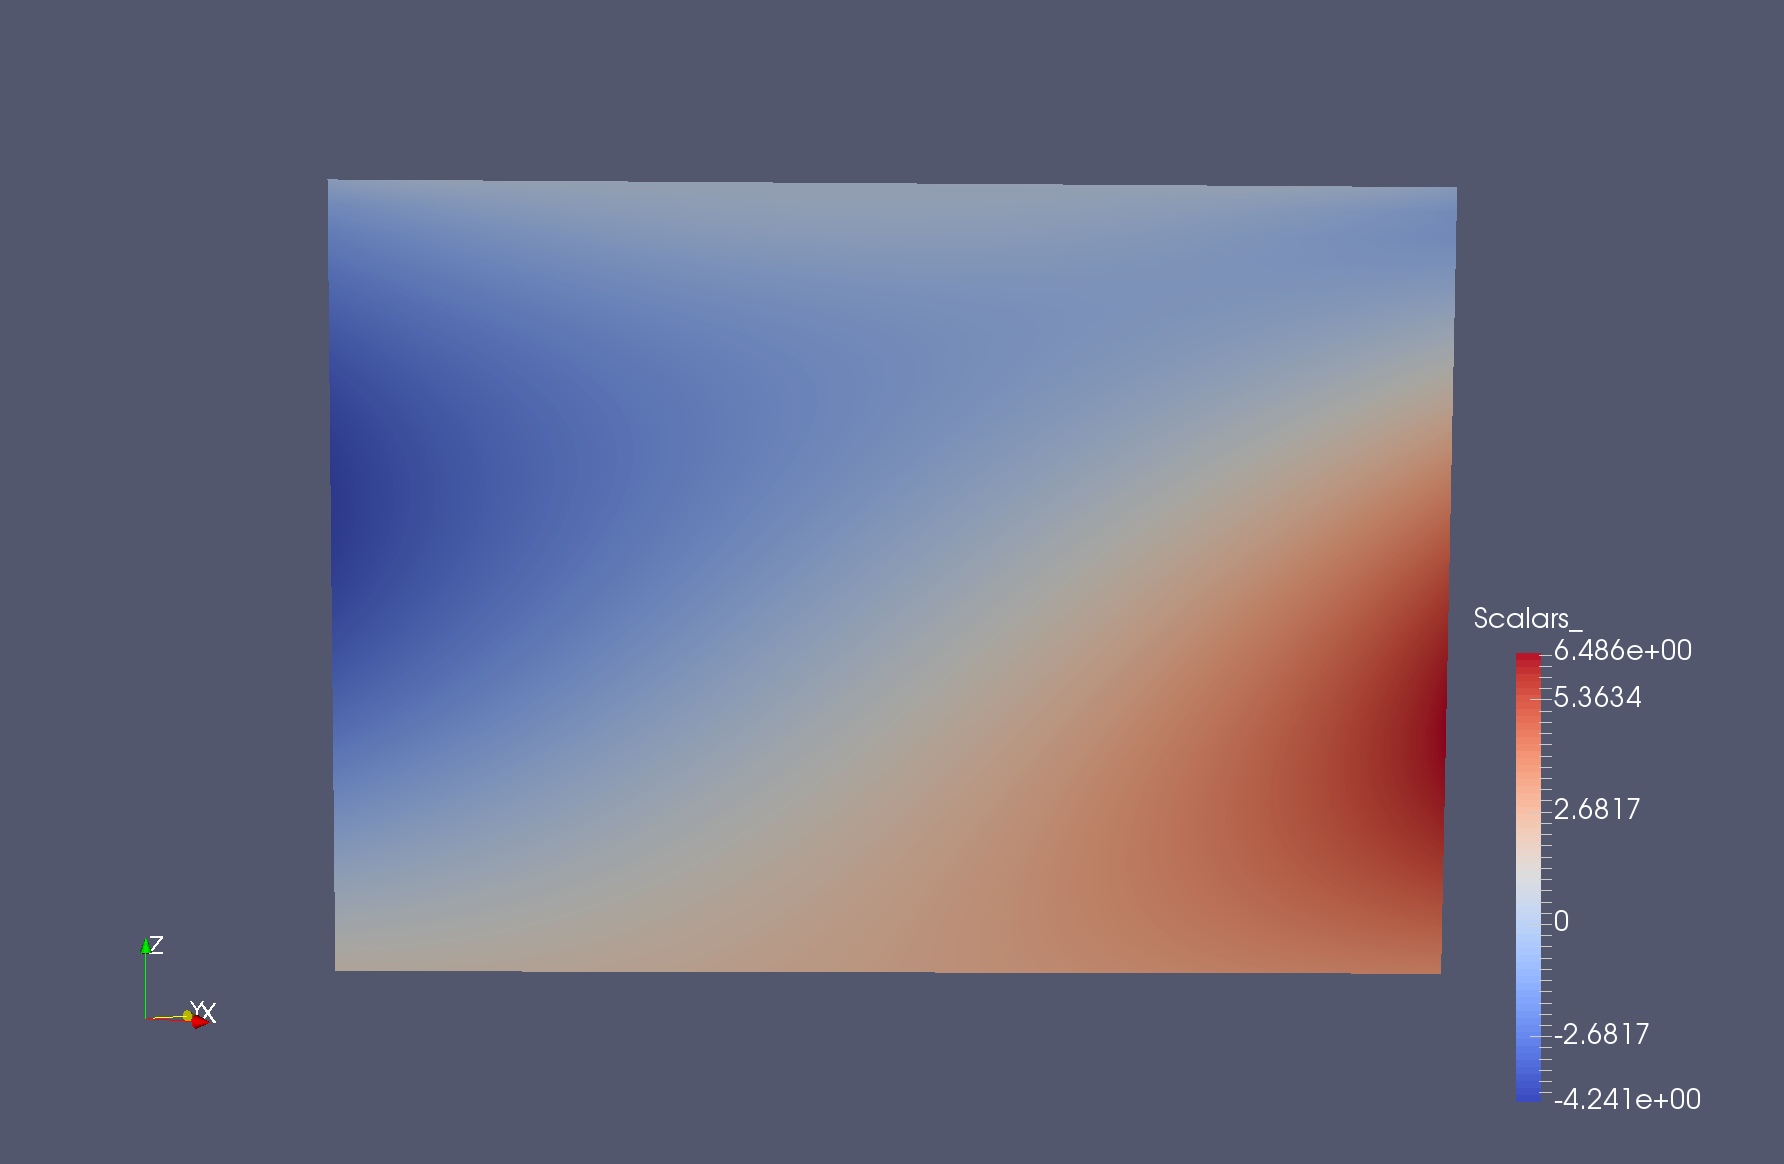
\includegraphics[width=0.9\textwidth]{Images/inner-u-cut-diag.png}
\caption{The optimal control of the inner control problem, plotted as a cut along the diagonal plane with normal $(-1, 1, 0)^\tp$ centered on $(0.5, 0.5, 0.5)^\tp$.}
\label{fig:inner-u-diag}
\end{figure}
\FloatBarrier

Of course, the implementation is not restricted to simple domains like the ones we've shown so far.
Using a quadratic domain for $\Omega$ was primarily done so that the results can be more easily visualized on paper.
As a next step, we will show some results for a different domain: Once again considering the inner heat source problem, with $y_Q$ as before, but scaled up by a factor $10$ for improved visibility, we now cut some part from the domain.
More specifically, we consider $\Omega = [0, 1]^2 \setminus [0.2, 0.8]^2$ and $T = 0.1$. This leaves us with a non-convex domain, which has a hole in its midst.
In \cref{fig:hole-y,fig:hole-u} we have given heat-maps of the optimal state and control on the space time domain $Q$, therefore showing a three dimensional plot this time.
As one can see, the lack of convexity in the domain itself matters little for the numerical method.
Do keep in mind however, that many regularity results for the parabolic heat equation depend on convexity of the domain.
\begin{figure}[htpb]
\centering
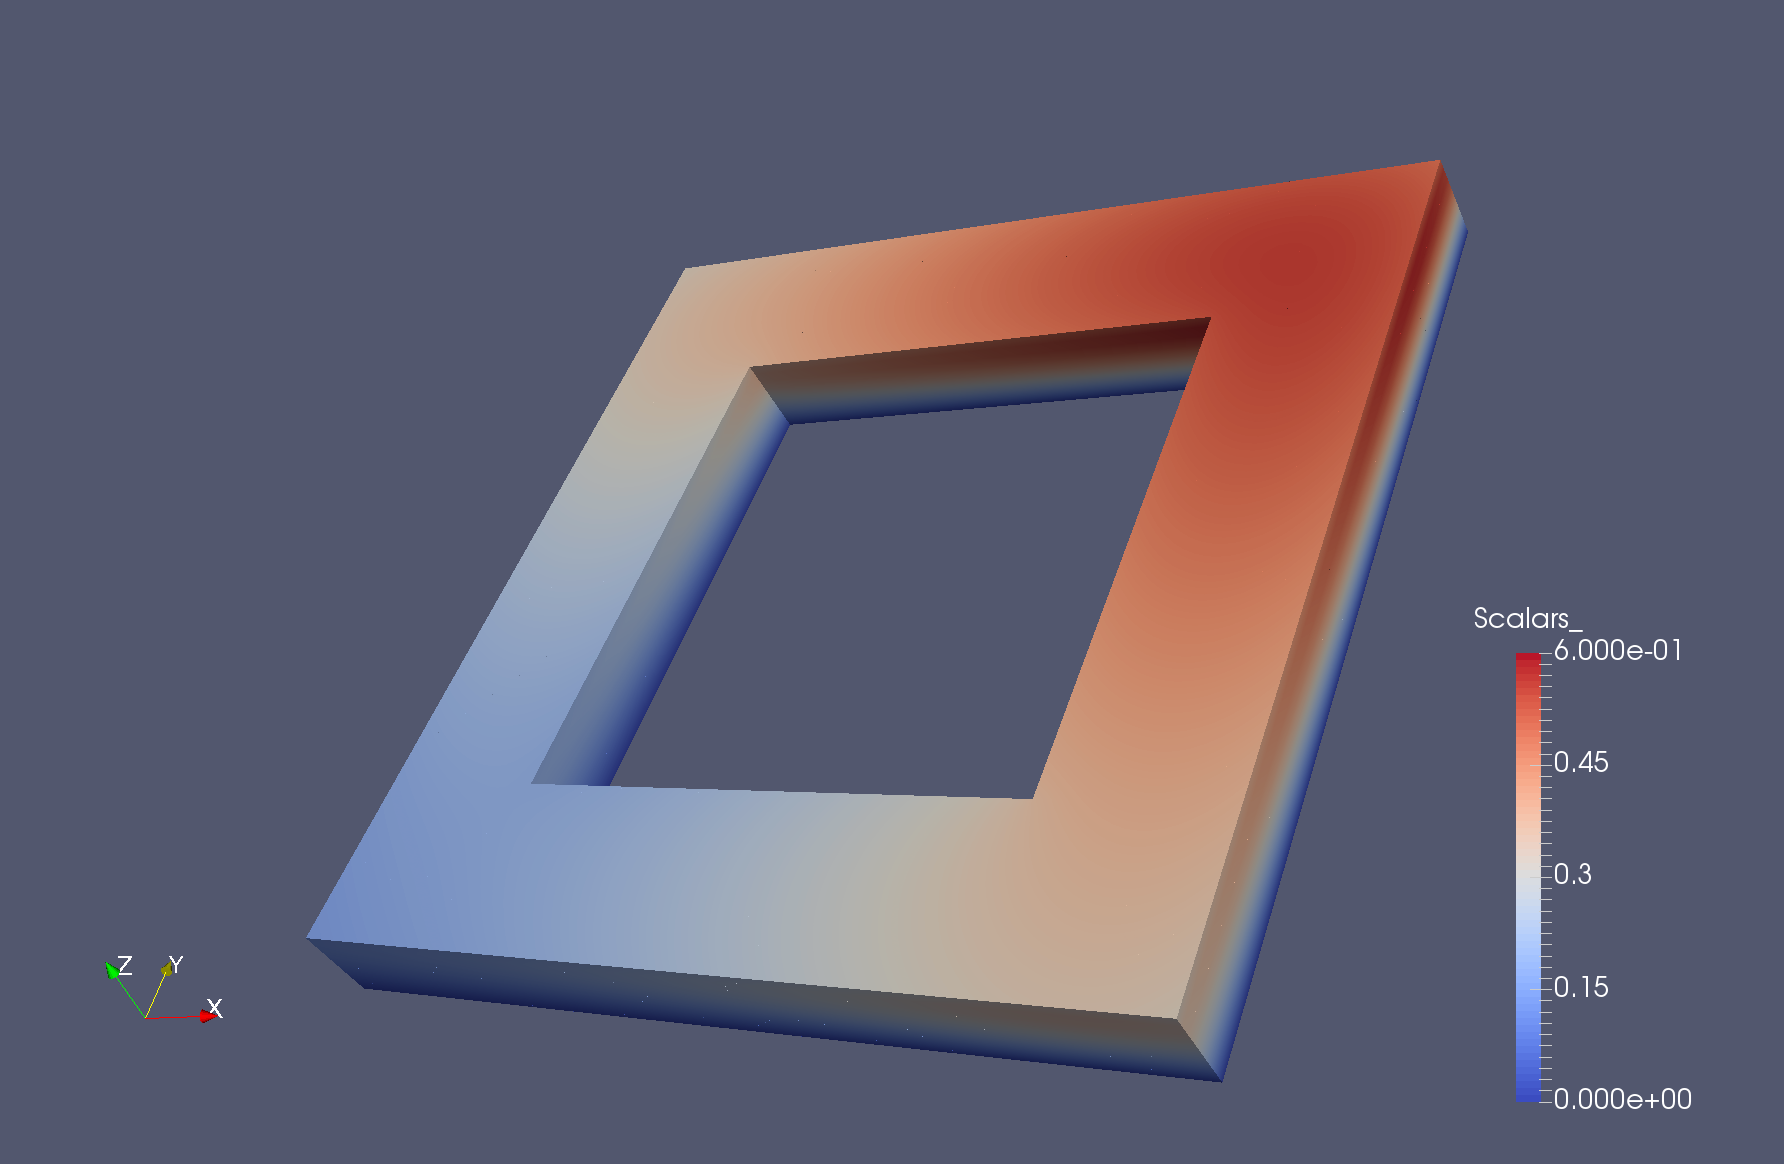
\includegraphics[width=0.9\textwidth]{Images/inner-hole-y.png}
\caption{The optimal state of the inner control problem with the new, cut out domain.}
\label{fig:hole-y}
\end{figure}
\begin{figure}[htpb]
\centering
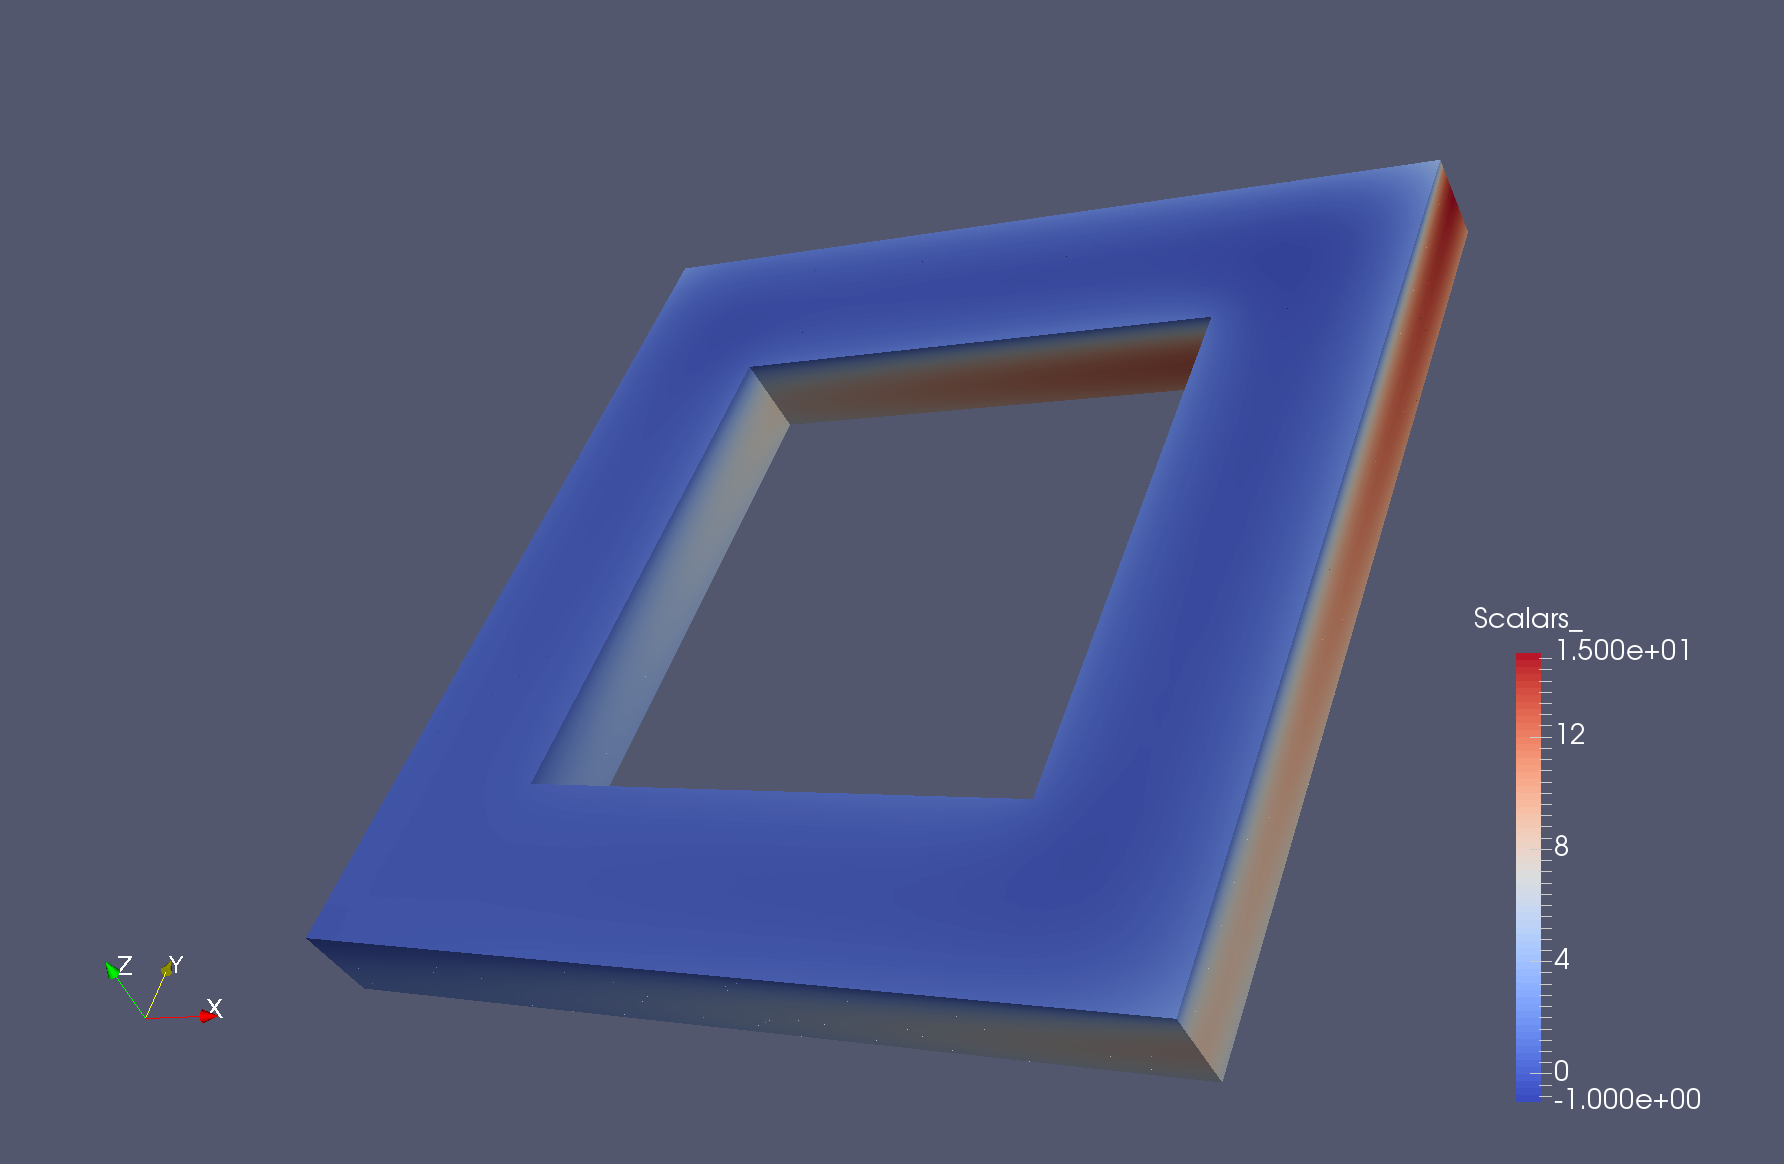
\includegraphics[width=0.9\textwidth]{Images/inner-hole-u.png}
\caption{The optimal control of the inner control problem with the new, cut out domain.}
\label{fig:hole-u}
\end{figure}
\FloatBarrier

All results so far were calculated by employing the sparse-direct solver PARDISO.
The reason for this is that iterative methods such as FGMRES converge poorly for the equation systems stem from the saddle point minimization problem.
We want to illustrate this with an example.
Consider again the unconstrained boundary optimal control problem for $y_0 \equiv 1$ and $y_\Omega \equiv 40$, which we discussed earlier.
\cref{fig:boundary-p} shows the adjoint state of the optimal control for this problem after three refinements.
If we attempt to solve the same linear equation system that stems from the discretization using a restarted variant of FGMRES, where we restart after 150 iterations, we obtain after 5000 iterations an iterate that is being shown in \cref{fig:GMRES-p}.
To be clear, \cref{fig:boundary-p} shows the exact solution of the linear equation system from which the iterate shown in \cref{fig:GMRES-p} stems.
One can clearly see that the unconditioned FGMRES method works poorly for solving the resulting linear system.

It is understood that the convergence of iterative methods including MINRES and GMRES\slash{}FGMRES depends critically upon the condition of the matrix.
The matrices that occur for the discretized optimal control problems are all of the form
\[
	\begin{pmatrix}
		M_1 & A_h^\tp \\
		A_h & M_2
	\end{pmatrix},
\]
where $A$ and $A^\tp$ are two matrices that are sparse but expected to be of rather benign form.
However, for the boundary optimal control problem, both $M_1$ and $M_2$ are mass matrices on boundary faces multiplied by some coefficients (for the inner optimal control problem, it is just $M_1$).
Therefore, neither can be invertible on their own.

Due to the absolutely critical dependence of the solution on both matrices, it's not surprising that the condition of the resulting system is rather poor.
After all, keep in mind that all the various problem formulations discussed here, use the same ansatz for the matrices $A_h$ and only differ by their choices for $M_1$ and $M_2$.

Ultimately, one would need a suitable matrix preconditioner if one wants to apply iterative methods to the resulting linear systems. The work \cite{BenziGolubLiesen} discusses several types of preconditioners suitable for saddle point problems like the ones encountered here.
Yet, they assume that the blocks $M_1$ or $M_2$ would be invertible, which they clearly cannot be in this case.
One might experience some success with block diagonal preconditioners for the systems resulting from the problem discussed in \cref{sec:symmetric-Problem} as both $M_1$ and $M_2$ are mass matrices stemming from the $L^2$ scalar product on $\Shp(\meshT_N)$ and therefore invertible.
Possibly such an approach could also be made for the inner optimal control problem from \cref{sec:inner-optimal-control}, where only $M_2$ is of full rank.
\begin{figure}[htpb]
\centering
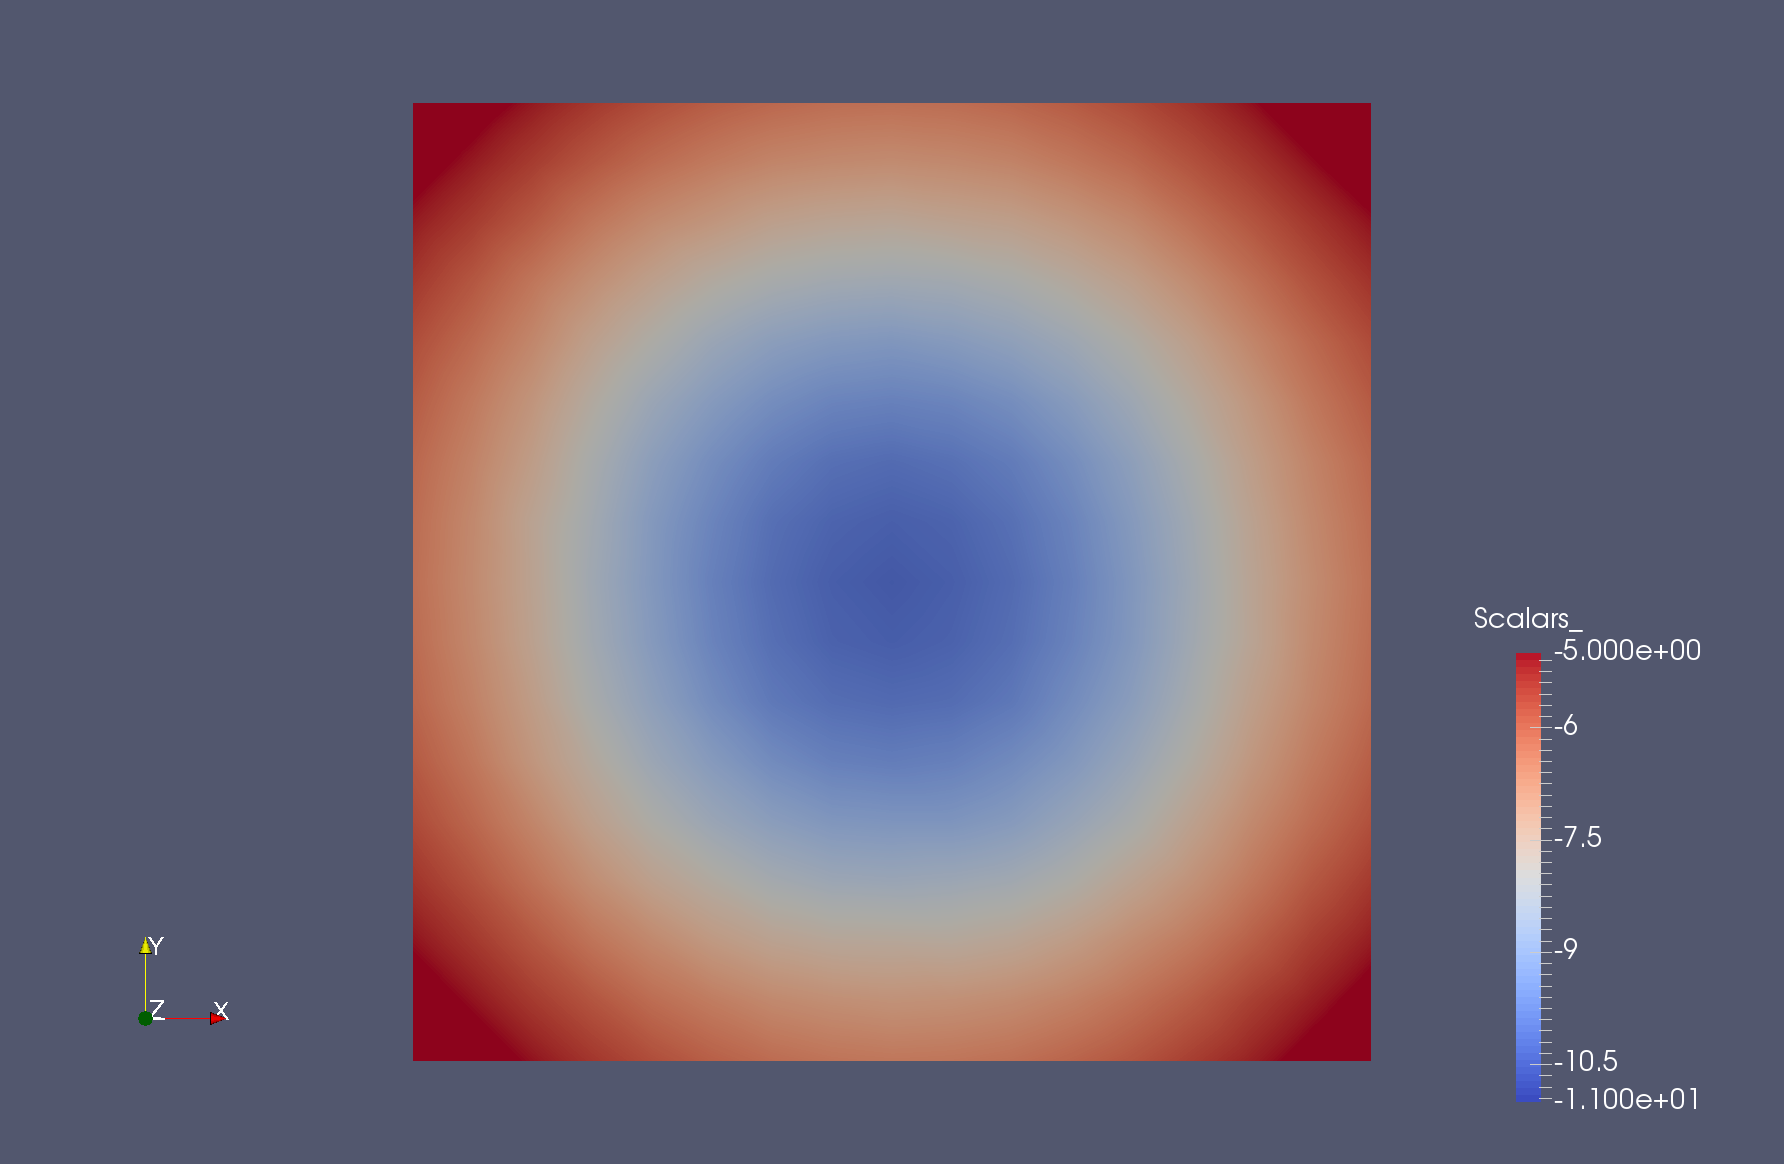
\includegraphics[width=0.9\textwidth]{Images/boundary-cont-p.png}
\caption{The optimal adjoint state of the boundary control problem for $y_0 \equiv 1$ and $y_\Omega \equiv 40$, plotted at $t = T$.}
\label{fig:boundary-p}
\end{figure}
\begin{figure}[htpb]
\centering
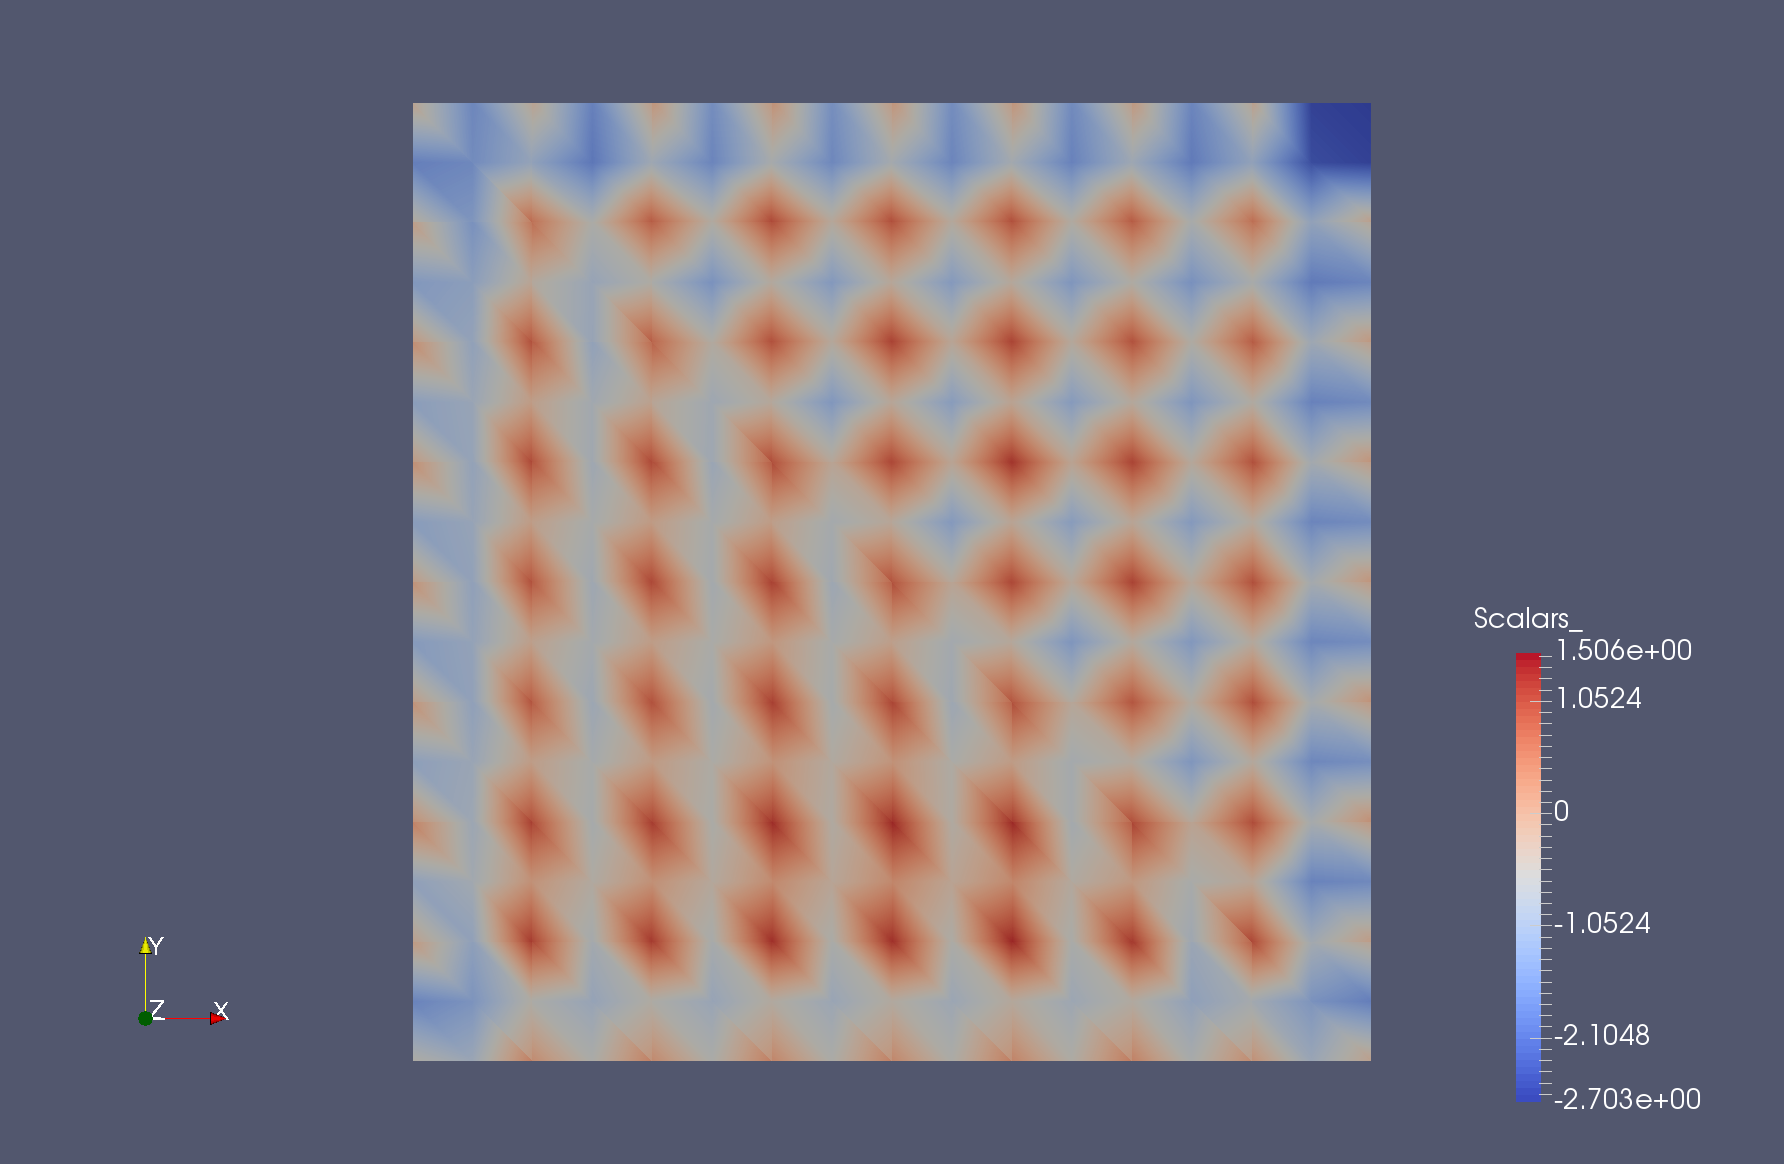
\includegraphics[width=0.9\textwidth]{Images/boundary-cont-GMRES.png}
\caption{The iterate of restarted FGMRES after 5000 corresponding the adjoint state of the boundary control problem for $y_0 \equiv 1$ and $y_\Omega \equiv 40$ as, plotted at $t = T$.}
\label{fig:GMRES-p}
\end{figure}
\FloatBarrier
\end{document}